\documentclass{sigchi}
%\documentclass{sig-alternate-10pt}


% llt: Define a global style for URLs, rather that the default one
%\makeatletter
%\def\url@leostyle{%
%  \@ifundefined{selectfont}{\def\UrlFont{\sf}}{\def\UrlFont{\small\bf\ttfamily}}}
%\makeatother
%\urlstyle{leo}


% To make various LaTeX processors do the right thing with page size.
\def\pprw{8.5in}
\def\pprh{11in}
\special{papersize=\pprw,\pprh}
\setlength{\paperwidth}{\pprw}
\setlength{\paperheight}{\pprh}
\setlength{\pdfpagewidth}{\pprw}
\setlength{\pdfpageheight}{\pprh}



\usepackage{graphicx}
\usepackage{epstopdf}
\usepackage{balance}
\usepackage{comment}
\usepackage{times,epsfig,subfigure,endnotes,color,url,paralist,multirow,float}
\usepackage[lined,ruled,linesnumbered,vlined]{algorithm2e}
\usepackage{cite}
\usepackage{verbatim}

% Make sure hyperref comes last of your loaded packages,
% to give it a fighting chance of not being over-written,
% since its job is to redefine many LaTeX commands.
\usepackage[pdftex]{hyperref}
\hypersetup{
    pdftitle={SIGCHI Conference Proceedings Format},
    pdfauthor={LaTeX},
    pdfkeywords={SIGCHI, proceedings, archival format},
    bookmarksnumbered,
    pdfstartview={FitH},
    colorlinks,
    citecolor=black,
    filecolor=black,
    linkcolor=black,
    urlcolor=black,
    breaklinks=true,
}

% create a shortcut to typeset table headings
\newcommand\tabhead[1]{\small\textbf{#1}}

\newcommand{\superscript}[1]{\ensuremath{^{\textrm{#1}}}}
\def\sharedaffiliation{\end{tabular}\newline\begin{tabular}{c}}

\def\winlab{\superscript{\dag}}
\def\cmu{\superscript{$\ast$}}
\def\ut{\superscript{\S}}
%\def\cornell{\superscript{$\star$}}

\makeatletter
\let\@copyrightspace\relax
\makeatother


\begin{document}

\title{Whose Move is it Anyway? Authenticating Smart Wearable Devices Using Unique Head Movement Patterns}

\numberofauthors{1}
\author{
 \\
 \\
 \\
 \\
 \\
}


\begin{comment}
\numberofauthors{1}
\author{
\alignauthor
 Sugang Li\winlab, Ashwin Ashok\cmu, Yanyong Zhang\winlab, Chenren Xu\cmu, Macro Gruteser\winlab, Janne Lindqvist\winlab\\
\vspace{4mm}
        \affaddr{{\winlab}WINLAB, Rutgers University, North Brunswick,NJ, USA}\\
          \vspace{1mm}
        \affaddr{{\cmu}Carnegie Mellon University, Pittsburgh, PA, USA}\\
}
\end{comment}

%\numberofauthors{1}
%\author{
%\alignauthor
%Sugang Li\winlab, Ashwin Ashok\cmu, Yanyong Zhang\winlab, Chenren Xu\cmu, Macro Gruteser\winlab\\
%\vspace{4mm}
%        \affaddr{{\winlab}WINLAB, Rutgers University, North Brunswick,NJ, USA}\\
%          \vspace{1mm}
%        \affaddr{{\cmu}Carnegie Mellon University, Pittsburgh, PA, USA}\\
%}

\maketitle
% infer number of people, queue serving, traffic pattern,mood inference
% add comparison of time convergence of cell and point, RSS signatures for
%different phones, can we detect how many people when drive by? add wifi
%receiver part.
\newcommand{\systemname}{{\em Headbanger}}

\begin{abstract}
In this paper, we present the design, implementation and
user studies of a novel approach to authenticate
wearable devices users based on their unique behavioral patterns. We 
prototype an authentication system, dubbed {\em Headbanger} for
head-worn wearable devices by monitoring user's unique head-movement patterns 
in response to an external audio stimulus. 
Solutions today primarily rely on indirect authentication
mechanisms through the user's smartphone, which can be cumbersome and more 
susceptible to adversary intrusions. Biometric solutions, 
are subject to the availability of the specific sensors in the wearable unit. 
Using a head-worn personal imaging device as a running example and
through extensive experimental evaluation with 30 human subjects, we show
that our mechanism can authenticate users with an average acceptance rate of
95.1\% while keeping the average false acceptance rate of 3.9\%.

\end{abstract} 

%The recent years have seen a significant growth in popularity of
%smart wearable devices. This growth can be attributed to the advances in
%hardware miniaturization technology as well as economically affordable
%and energy efficient sensing and computing. While size, energy and cost
%constraints remain key motives for improvements in wearable computers'
%design, the aspect of user authentication has received relatively less
%attention. Wearable devices often collect and store sensitive data about
%users, and thus there is an obvious need to authenticate the right user to the
%device.
\section{Introduction}\label{sec:intro}

We live in a world that has seen a generation of technological revolutions;
from wired to wireless communications, immovable to mobile machines, large
sized to hand-held devices. Today, we are witnessing what can be deemed as the
next phase of mobile revolution through {\em wearable computers}. Research in
wearable computers can be dated back to as early as 1980s when Steve Mann
developed a prototype heads-up-display goggles~\cite{mann1997wearable}. Thanks to the
advances in hardware miniaturization technology, cheap sensors/processor
chips, and low-power sensing/computing, today, wearables are available
off-the-shelf and have almost become an integral part of human
lives~\cite{googleglass,smartwatch,fitbit}.

%This is clearly evident from the surge in the number and types of wearables
%that are commercially available -- ranging from smart glasses, smart
%necklaces, smart wristbands, to smart watches.
The surge in wearables is clearly seen commercially through the array of
smart wearable devices seeping fast into the market. Research on wearables has
actively picked up and is progressing over the day. Keeping in mind the
resource limitations on wearable computers research so far has primarily
been addressing three key optimization parameters in
design: size, energy and cost. With the onset of proliferation of wearable
devices, in the recent times the aspect of security and privacy have also been
adding key concerns to wearable computer usage.
A solution for safeguarding the security and privacy of user's data on the
wearable device is only effective as long as the device itself is
authenticated to the right user/owner.

\begin{figure}
\centering
\includegraphics[width=\columnwidth]{fig/headbanger-illustrate.png}
\caption{Illustration of Headbanger. The head-worn device authenticates the
right user based on signatures generated from head-movement patterns in
response to an audio snapshot played on the device.}
\label{fig:headbanger-illustrate}
\end{figure}

\vspace{1mm}\noindent{\bf Authentication Challenge.}
%User-authentication for wearable devices has so-far received relatively less
%attention; commercially as well as in research.
Authentication on most commercially available wearable devices
today~\cite{fitbit, smartwatch} relies on an indirect mechanism, where users
can login to their wearables through their phones. This requires the wearable
device to be registered and paired to the user's mobile device, which makes it
inconvenient as the user has to carry both the devices. The security of this
approach is also in question as it increases the chance of hacking into
 both the devices if either of the devices are lost or stolen.
Some devices including Google Glass~\cite{googleglass} and
FitBit's health tracker~\cite{fitbit}, pair the device to the users email
account instead of the phone for user's convenience; however, it does not add any
security benefit. Though wearable devices today almost contain the same suite
of sensors as a smartphone, the computing capacity and battery lifetime of
wearables are far less comparable. This implies that, translating the same
 authentication solution from a phone to the wearable device, to enable
direct authentication, is not only undesirable but also impractical.
\emph{Thus, the need for the day is a simple, low-power, and accurate
direct authentication solution.}
%For example, fitness trackers and
%smart-watches are tethered to user's mobile device to connect to the
%Internet as well as for remote data collection.

There have also been a few specific point solutions that propose to directly
authenticate the user to the device using biometric signatures~\cite{rahman2014bodybeat,cornelius2014wearable}. However, collecting and recognizing these biometrics is subject
to the availability of the sensing hardware and the computing capability on
the wearable units, hence unrealistic in most
cases. The recent years have also seen a significant interest in using
behavioral characteristics of humans as biometric signatures for mobile phone
authentication~\cite{stevenage1999visual,okumura2006study,monrose2000keystroke,jorgensen2011mouse,bo2013silentsense,de2012touch}.
For example, human walking gait, arm swings, typing patterns, body pulse
beats, eye-blinks have all been found to be distinctive in human beings.
The main advantage of using behavioral biometrics is that the signatures can
be generated from raw data of basic sensor that are inbuilt in mobile phones
such as motion sensors, camera, microphones etc. However, what behavioral
biometric remains the best suited for a wearable device and if such a
biometric can be captured by the wearable device lays a fundamental question
for a system that may adopt this approach.

\vspace{1mm}\noindent{\bf Head-movement based authentication.}
In this paper, we propose to authenticate wearable devices to users based on
their unique behavioral patterns. Keeping in mind the feasibility of
implementation and the availability of the sensor on the wearable device,
we design a system that authenticates users to their device directly through
their head-movement patterns.
In particular, we prototype an authentication system, dubbed {\em Headbanger},
that generates a signature from user's head-movements that serves as the
behavioral biometric for authentication. To ensure that the user is proactive
in making head-movements we stimulate the process by playing a short duration
audio track with fast beats. The user in response to the rhythm and beats
makes head-movements that are captured by the accelerometer and processed to
generate and authenticate the user's unique biometric signature.
While we use a Google Glass a running example for the wearable device, our
design can be applied to other head-worn gadgets and any system that can
record head-movements through motion sensing.
Our choice for using head movements is motivated by the fact that head-worn
wearables are becoming very common today and such devices are already equipped
with motion sensors; for example, personal imaging and heads-up display
devices, gaming headsets, AI devices.

%Unlike physiological biometrics that require custom hardware,
%behavioral biometrics offer a much more available/conveient solution. The
%challenge, however,
%is to ensure that these patterns are repeatable under all circumstances that
%the user encounters as well as the differentiability factor between different
%human beings. %We show that by using the same external stimulus among all
%%users
%the baseline for comparison is achieved much easier and the head-patterns are
%more consistent and differentiable among users.

%Subconscious head-movement, or any body movement as a matter
%of fact, can be very random in general.
% Our design assumes that there is only one owner per glass, and we can easily
%extend our scheme to handle the cases with multiple owners.

In summary, the key contributions of this paper are:

\begin{enumerate}

\item We propose a technique for direct authentication to wearable devices
using head-movement patterns. We show that user's head-movement patterns
contain unique signatures that when inferred correctly can be used as valid
behavioral biometrics for authentication.

\item We design an authentication system, \systemname,~ that records,
processes, generates unique signatures, and classifies head-movement patterns
of users based on the accelerometer (inbuilt on the wearable device) sensor
readings.

\item We devise of a set of light-weight preprocessing and classification algorithms that can effectively transform raw and noisy sensor data into accurate authentication results. We aggressively optimize the processing latencies of these algorithms so that they are well suited for wearable devices.

\item We implement a data collection application on Google Glass that plays a
fast beat music (preloaded) through the Glass's speakers and simultaneously
records and filters accelerometer sensor data. We use this data collection app
in our experiments to evaluate the system.

\item Through extensive experiments involving multiple users\footnote{Our
human user experiments were approved by Rutgers University IRB} and over
different system design parameters we have shown that head-movement patterns
can be used as a
valid behavioral biometric.
To effectively identify a smart wearable device user,
with average false acceptance rate of 4.9\% and average false rejection rate
of 3.9\%.

\item We have conducted detailed validation of using head-movement patterns as a biometric characteristic by collecting and analyzing data from multiple users. We will make these data publicly available, which may facilitate other user behavior studies.
\end{enumerate}

In the sections to follow, we will discuss the background of wearable
device authentication in section~\ref{sec:background} and details of our
proposed system design in section~\ref{sec:design}. We evaluate the system in
section~\ref{sec:results} and follow up with discussions and conclusions in
sections~\ref{sec:disc} and \ref{sec:conc}, respectively.












\iffalse
Wearable devices are typically user-interface constrained
Unlike a smartphone, touch gestures or voice activation or face
recognition units not all wearable devices today have the generic
user interfaces such as touch or audio or visual so that typical
gesture or

The recent years have seen a significant growth in popularity of
smart wearable devices. This growth can be attributed to the advances in
hardware miniaturization technology as well as economically affordable
and energy efficient sensing and computing. While size, energy and cost
constraints remain key motives for improvements in wearable computers'
design, the aspect of user authentication has received relatively less
attention. Wearable devices often collect and store sensitive data about
users, and thus there is an obvious need to authenticate the right user to the
device. Solutions today primarily rely on indirect authentication
mechanisms through the user's smartphone, which can be cumbersome and less
secure. Biometric based solutions, though very effective, however, are subject
to the availability of the specific sensors in the wearable unit. In this
paper, we propose to authenticate wearable devices to users based on their
unique behavioral patterns. In particular, we prototype an authentication
system for wearable devices by monitoring user's unique head-movement patterns
in response to an external audio stimulus. Using a personal imaging device as
a running example, and through extensive experimental evaluation over multiple
users, we show that our mechanism can authenticate users with high accuracy


\fi 
\section{Background}
\label{sec:background}

\subsection{Wearable Device Authentication}


%\begin{comment}

%\end{comment}

%Authentication mechanisms for wearable devices can broadly be divided into two
%categories: (i) {\em Direct} authentication, where the users can directly
%authenticate themselves to their wearable device using the input/output
%interface and/or using signatures generated from the sensors available on the
%device, and (ii) {\em Indirect} authentication, where a secondary device --
%typically the user's smartphone -- is used as a medium for authentication.
%Today's commercially available wearable devices predominantly use the latter
%approach where users login to their wearable devices through their smartphone
%-- using a PIN or an email account.  
%%A select few gadgets, for example the Google Glass or fitbit, require the
%%users to register their device to their user specific accounts (gmail for
%%Google Glass), which can also be perceived as an indirect mechanism for
%%authentication.
%Unlike the indirect approaches, that require users to have multiple devices, direct
%mechanisms only rely on the wearable device by leveraging the inbuilt interfaces and sensors on the
%wearable device.

%%One form of direct authentication is the well-known
%%the PIN code approach, however, its effectiveness is only limited to the PIN
%%being safe-guarded by the user. A slightly more effective approach would be
%%to use a randomly generated code for the user, similar to the RSA
%%%keys~\cite{},but that would require a secure and stable wireless connection
%%%to the server.
%The fact that wearable devices relate significantly to ``what we wear" on the
%human body, biometrics can play a key role for direct authentication to
%wearable
%devices. 

Biometrics allow a system to identify a user based upon ``who you
are" (i.e., her physiology) instead of ``what you
have'' (i.e., ID cards) or ``what you know'' (i.e.,
passwords)~\cite{jain2004introduction,o2003comparing,yampolskiy2007motor}.
Physiological biometrics such as DNA, ear shape, face, fingerprint,
hand or finger geometry,
iris, odor, palm-print, retinal scan, and voice, have been very effective and
widely used in many prototype and commercial authentication systems.
In addition, body shape such as body height, width, and body-part proportions
can also be used as biometric cues to identify different
people~\cite{collins2002silhouette}. Even characteristics such as
body weight and fat percentage have been considered as secondary biometrics
for authentication purposes~\cite{ailisto2006soft}. 

However, biometrics are
not prominently used in wearable devices that are commercially available 
today, though
there have been specific point commercial designs (e.g., Nymi~\cite{nymi}). This can be attributed to the
fact that biometrics would require the specific hardware and sensors available on
the wearable device. Also the overheads for physiological biometrics in
wearable devices can be high, in both, cost for hardware as well as
integration and computing.

%Most of the afore-mentioned biometrics, however, require extra hardware
%(e.g., camera) and/or processing that is too demanding for wearable devices.

An other approach to direct authentication is using behavioral biometrics
where unique signatures from human behavior (subconscious
or in response to external stimulus) provide cues for differentiating and
authenticating users. For example, it has been shown that gait (e.g.,
stride length, the
amount of arm swing) when the user is walking or
running is a reliable identification cue, and irrespective of the
environment~\cite{stevenage1999visual}. Okumura et.al.~\cite{okumura2006study}
have shown that the human arm swing patterns can be used to create signatures
to authenticate to their cell-phones. Monrose
et.al.~\cite{monrose2000keystroke} show that keystroke rhythms, when
users type on the keyboard, that include typing dynamics such as how
long is a keystroke, how far is between consecutive strokes, and how is the
pressure exerted on each key, can be used as a biometric to authenticate
users. Similarly, mouse usage dynamics~\cite{jorgensen2011mouse} and touchpad
touching dynamics~\cite{bo2013silentsense,de2012touch} have also been shown to
serve as potential biometrics.

In comparison to other means of authentication, behavioral biometric
authentication can offer a more convenient (than physiological biometrics),
and more secure (than indirect authentication) solution for wearable device
authentication. With the increasing off-the-shelf
availability and (almost) unlimited access to the sensors on the wearables, it
has become possible to generate and infer unique behavioral signatures
specific to users. We use these rationale as a motivation for our proposed
design of a behavioral biometric based authentication that generates unique
signatures from accelerometer signal patterns from user's head movements.
We design an authentication system, dubbed {\em Headbanger}, for head-worn
devices by monitoring user's unique head-movement patterns in response to an
external audio stimulus.

%\vspace{4pt}{\bf Head-movements as a behavioral biometric.}
\subsection{Head-movement as a Biometric}
\label{subsec:headmovements}

%As such, authenticating a user involves comparing her sensor
%readings with the pre-recorded glass owner's sensor readings.
%Our design assumes that there is only one owner per glass, and we can easily
%extend our scheme to handle the cases with multiple owners.
%Figure~\ref{fig:sysarch} presents the system architecture of the \systemname,
%and in the following section, we will discuss each component of this design
%in more detail.

According to Jain et al.~\cite{jain2004introduction}, a human characteristic can be
considered as biometric as long as it is \emph{universal}, \emph{distinctive},
\emph{repeatable}, and \emph{collectible}. With the advancements in head-worn
wearable computer designs collecting head-movement
patterns using the built-in accelerometers and motion sensors has become more 
accessible. Such sensors are
available on almost all head-worn wearable devices available today, thus
making head movements, both, available {\em universal} and \emph{collectible}. 

In this paper, we will show that free-style head movements are \emph{distinctive} and \emph{repeatable}, especially when combined with external stimuli such as music. In~\systemname, music plays a crucial role in stimulating body movements such that the resulting movement pattern is natural to the user (more distinctive) and easier to remember (more repeatable). It has been shown~\cite{zentner2010rhythmic} that most people move
their body as a natural response to external rhythmic stimuli such as music;
even at a very early age, infants respond to music and their movements speed
up with the increasing rhythm speed. Most adults naturally perform head 
movements or hand movements when listening to a fast beat audio track.  When 
combined with external rhythmic stimuli, we believe body movements become more 
distinctive -- not only a person's movement pattern is unique, but their 
response to rhythmic stimuli is also unique. In this way, the resulting 
authentication system will be more dependable.

Based on a
preliminary analysis of the accelerometer signals from five Google Glass
users, we also observed (see Figure~\ref{fig:raw} (a)-(e)) 
that these users
{\em repeatedly} showed unique and {\em distinctive} head-movement patterns 
(that are differentiable through simple signal processing techniques),
when listening to the same music beats on the head-worn device.
Motivated by this observation we hypothesize that head movements
can be a good behavioral biometric characteristic to authenticate
users to their smart glass.
We next formally present the design of our system that
utilizes head-movement patterns as behavioral biometric signature
to authenticate smart glass users.

\begin{figure*}[t]
\begin{center}
\begin{tabular}{ccc}
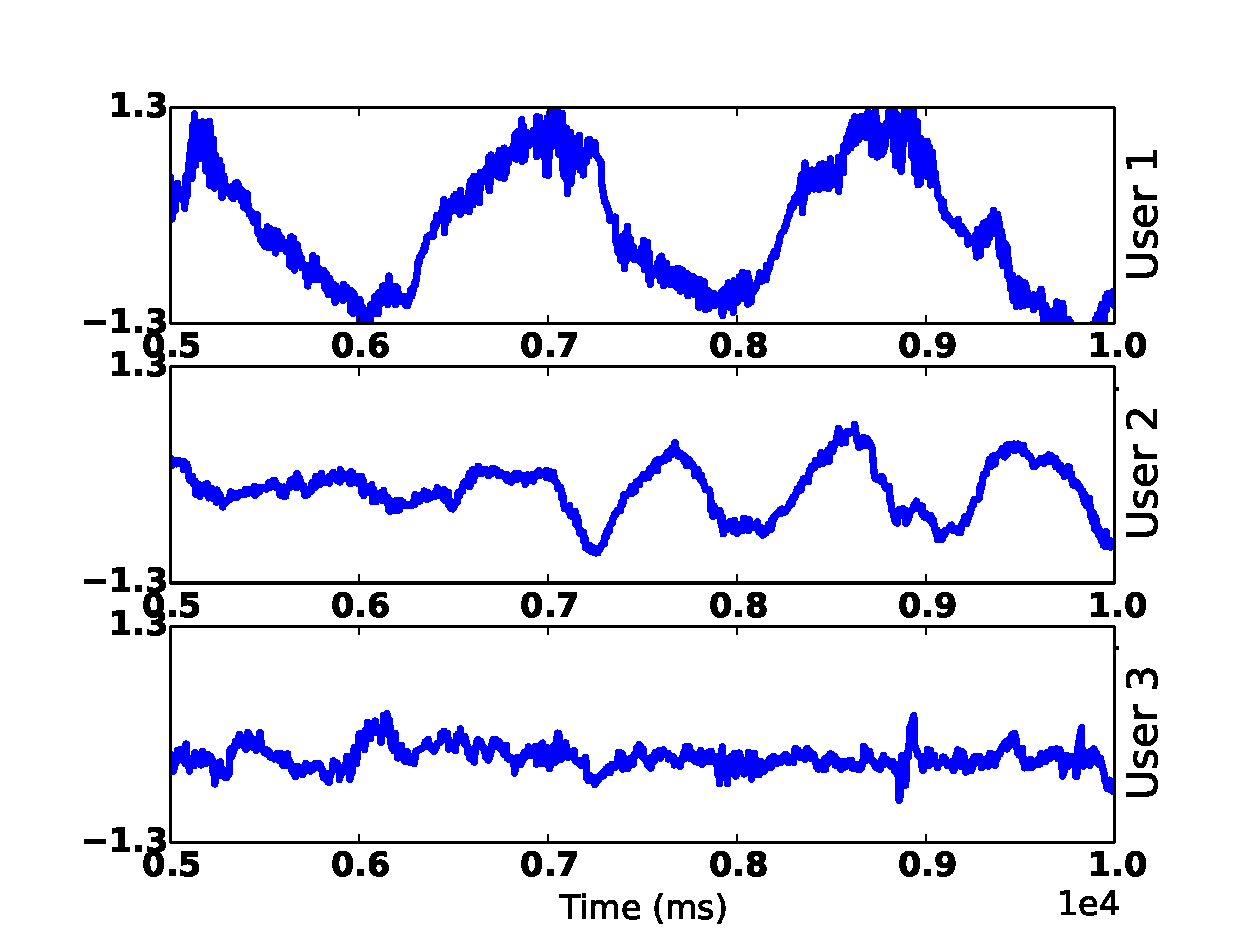
\includegraphics [width=.33\linewidth]{figure/raw_x.eps}&
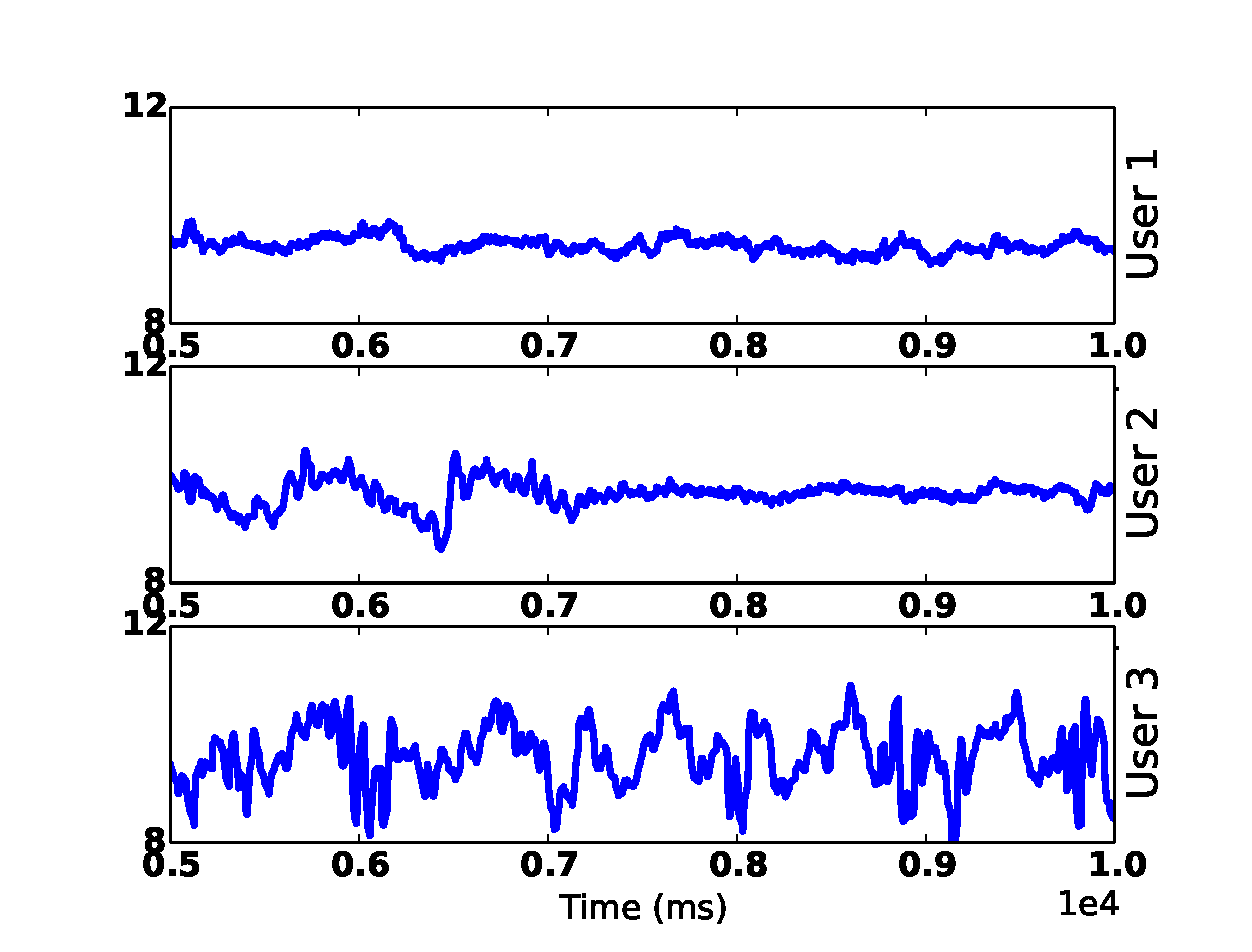
\includegraphics [width=.33\linewidth]{figure/raw_y.eps}&
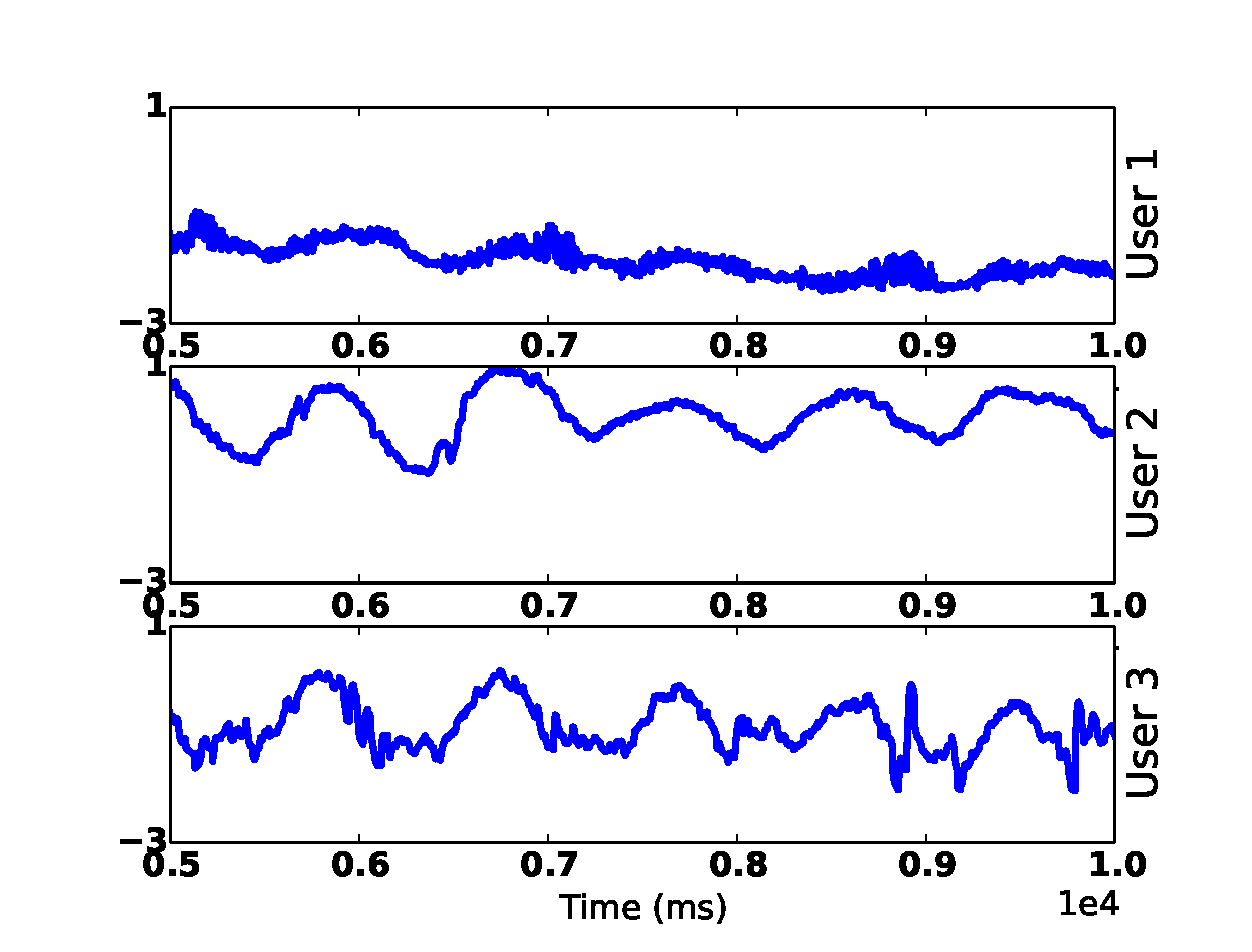
\includegraphics [width=.33\linewidth]{figure/raw_z.eps}\\
(a) X-Axis & (b) Y-Axis & (c) Z-Axis \\
\end{tabular}

%\begin{tabular}{cc}
%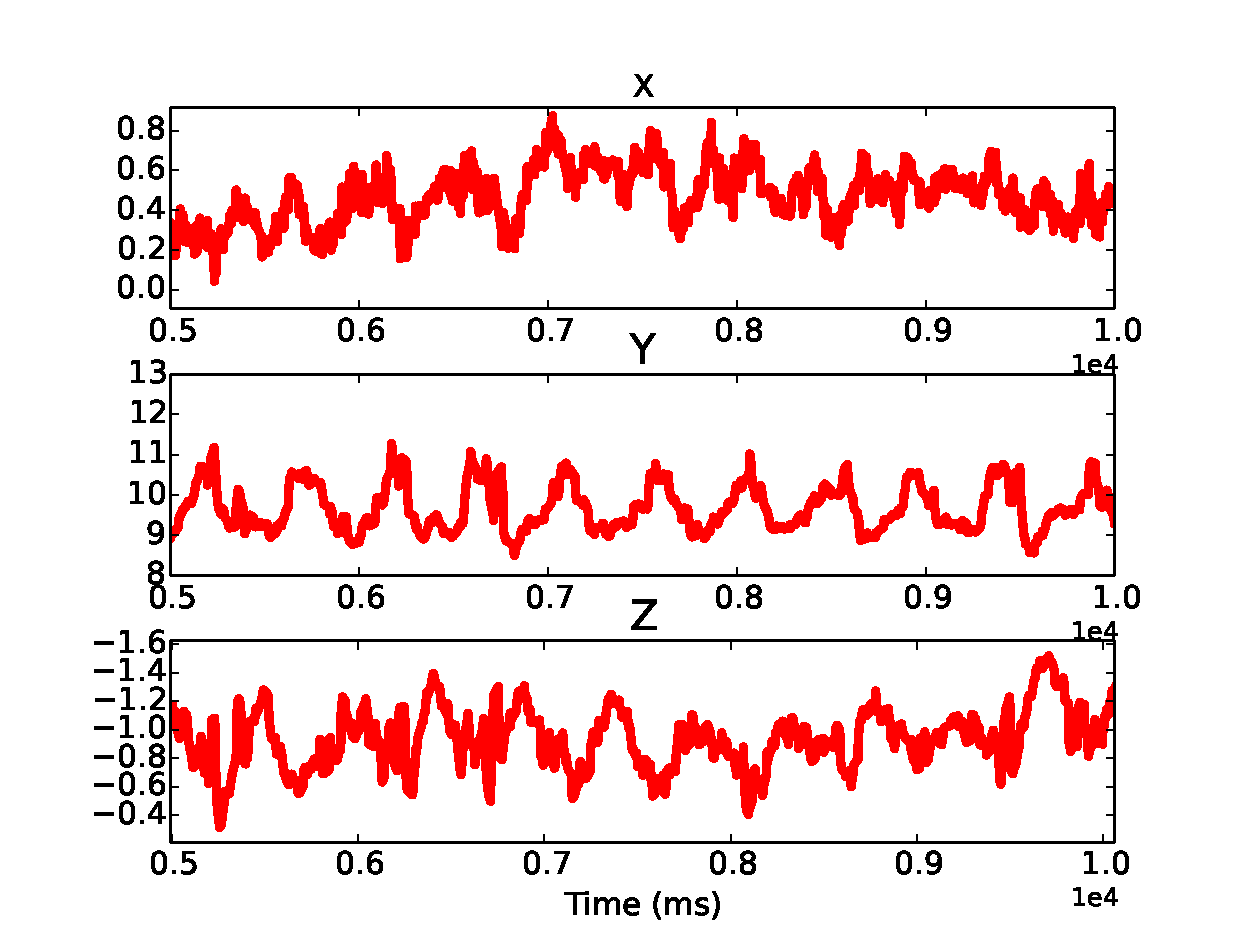
\includegraphics [width=.33\linewidth]{../fig/raw_sub4.eps}&
%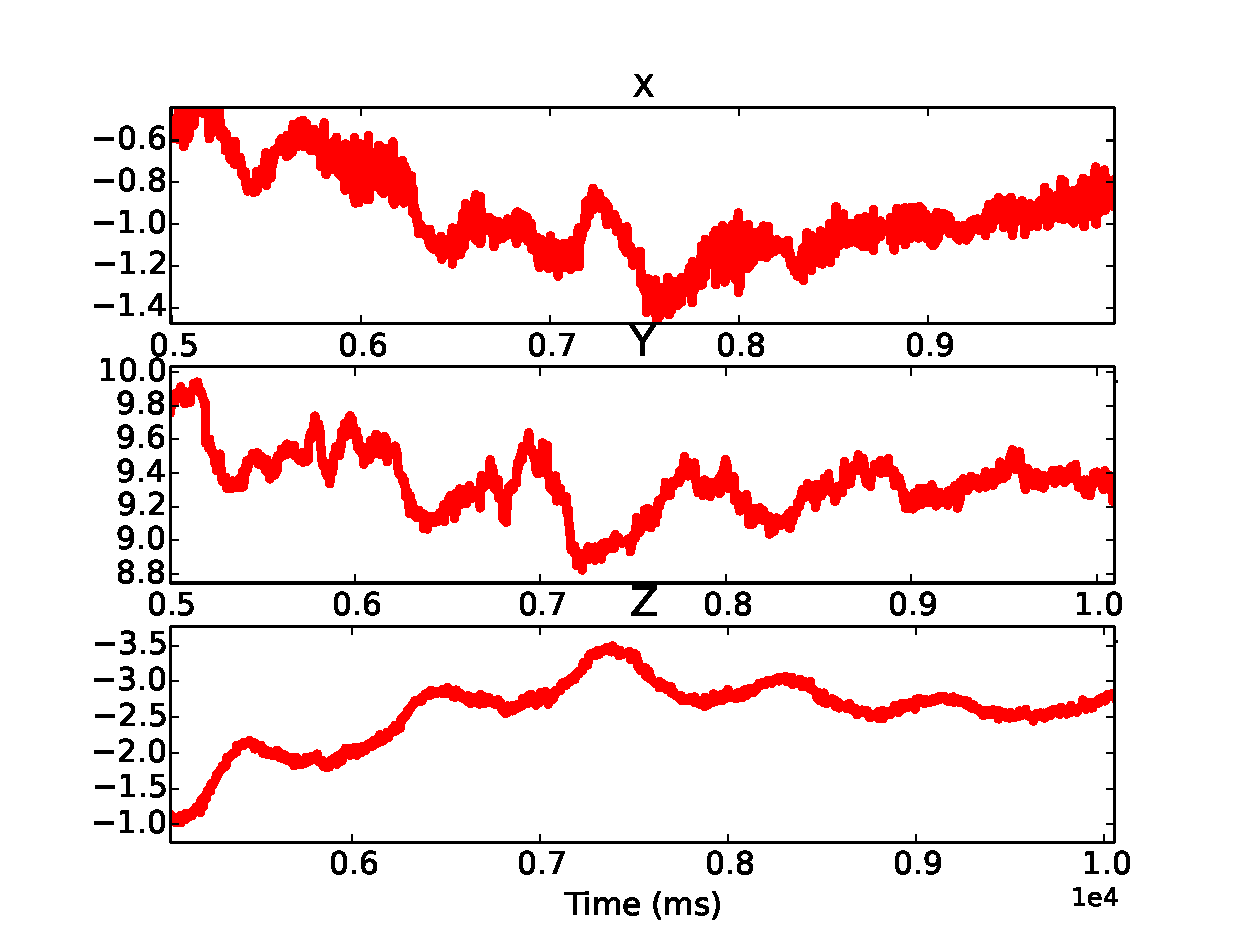
\includegraphics [width=.33\linewidth]{../fig/raw_sub5.eps}\\
%(d) User 4& (e) User 5 \\
%\end{tabular}
\end{center}
\caption{\label{fig:raw} These plots show the raw accelerometer data in the
time domain for five different users when they move their head in response to
the same music track wearing the same Google glass. The plots
indicate that different users' head movement patterns appear distinctive from
each other. The three users wore a Google Glass (in turns) and listened to a
10 second audio snapshot of a pop song.}
\vspace{-2pt}
\end{figure*}
\section{Preliminary Study}
In order to understand the insightful information of musical head movement, we conducted a experiment to collect head-movement accelerometer data from 28 subjects(** LS:Do we need to mention IRB here?**). Each subject was asked to perform simple nodding movement by following the music cue.  We extract several characteristics from the original accelerometer data:
\begin{itemize}
\item{\em Wave amplitude},which is the difference of a wave bottom and its next wave peak. It measures the acceleration when the user performs the head-movement, in other words, wave amplitude describes “how hard” the user nod his head. Due to accelerometer data usually contains high frequency noise, and we are more interested in the main signal where user nod his head, a 5-Hz-cutoff low-pass filter is applied before we extract all the characteristic in the signal.   
\item{\em Wave widh}, which is the time interval between two bottoms or two peaks. It describes the time to complete one nodding movement. The user is stimulated by a music cue, wave width is effected by the time interval between beats.
\item{\em Series of response time (SRT)},which is the series of time interval between the music beat and corresponding movement.  Studies in ~\cite{westeyn2004recognizing} and ~\cite{wobbrock2009tapsongs} show SRT could be used to differentiate the users. It is important to note that user is not necessary perform after the music beat. The evidence in music psychology ~\cite{clarke1999rhythm,fraisse1982rhythm} demonstrate that  humans have capability to perceive and perform rhythmm, hence user can perform the moving before he hears the beat.
response time in our measurement can be either negative or positive. However, finding the associated movement of a beat is a non-trivial process, hence we develop the following algorithm to achieve this goal and form a SRT. First, accelerometer data needs to be synchronized with the music cue in midi format. Since midi file is a time series of instrument commands,  no additional signal processing is required to detect the beat in the music as we can take each command as a beat if the music is simple enough. Second, we locate two neighboring peaks where a beat resides in between, and compute the time intervals from the beat to both peaks. Finally, we choose the one with a smaller absolute value as the response time. Note that we only use data from two axis, since nodding rarely generates meaningful data on the other one. In some cases,  user is not necessary nodding for every beat,  thus we use the 90 percentile of the response time sample to interpolate  when the detected response time is beyond this value. 
\end{itemize}
\begin{figure}
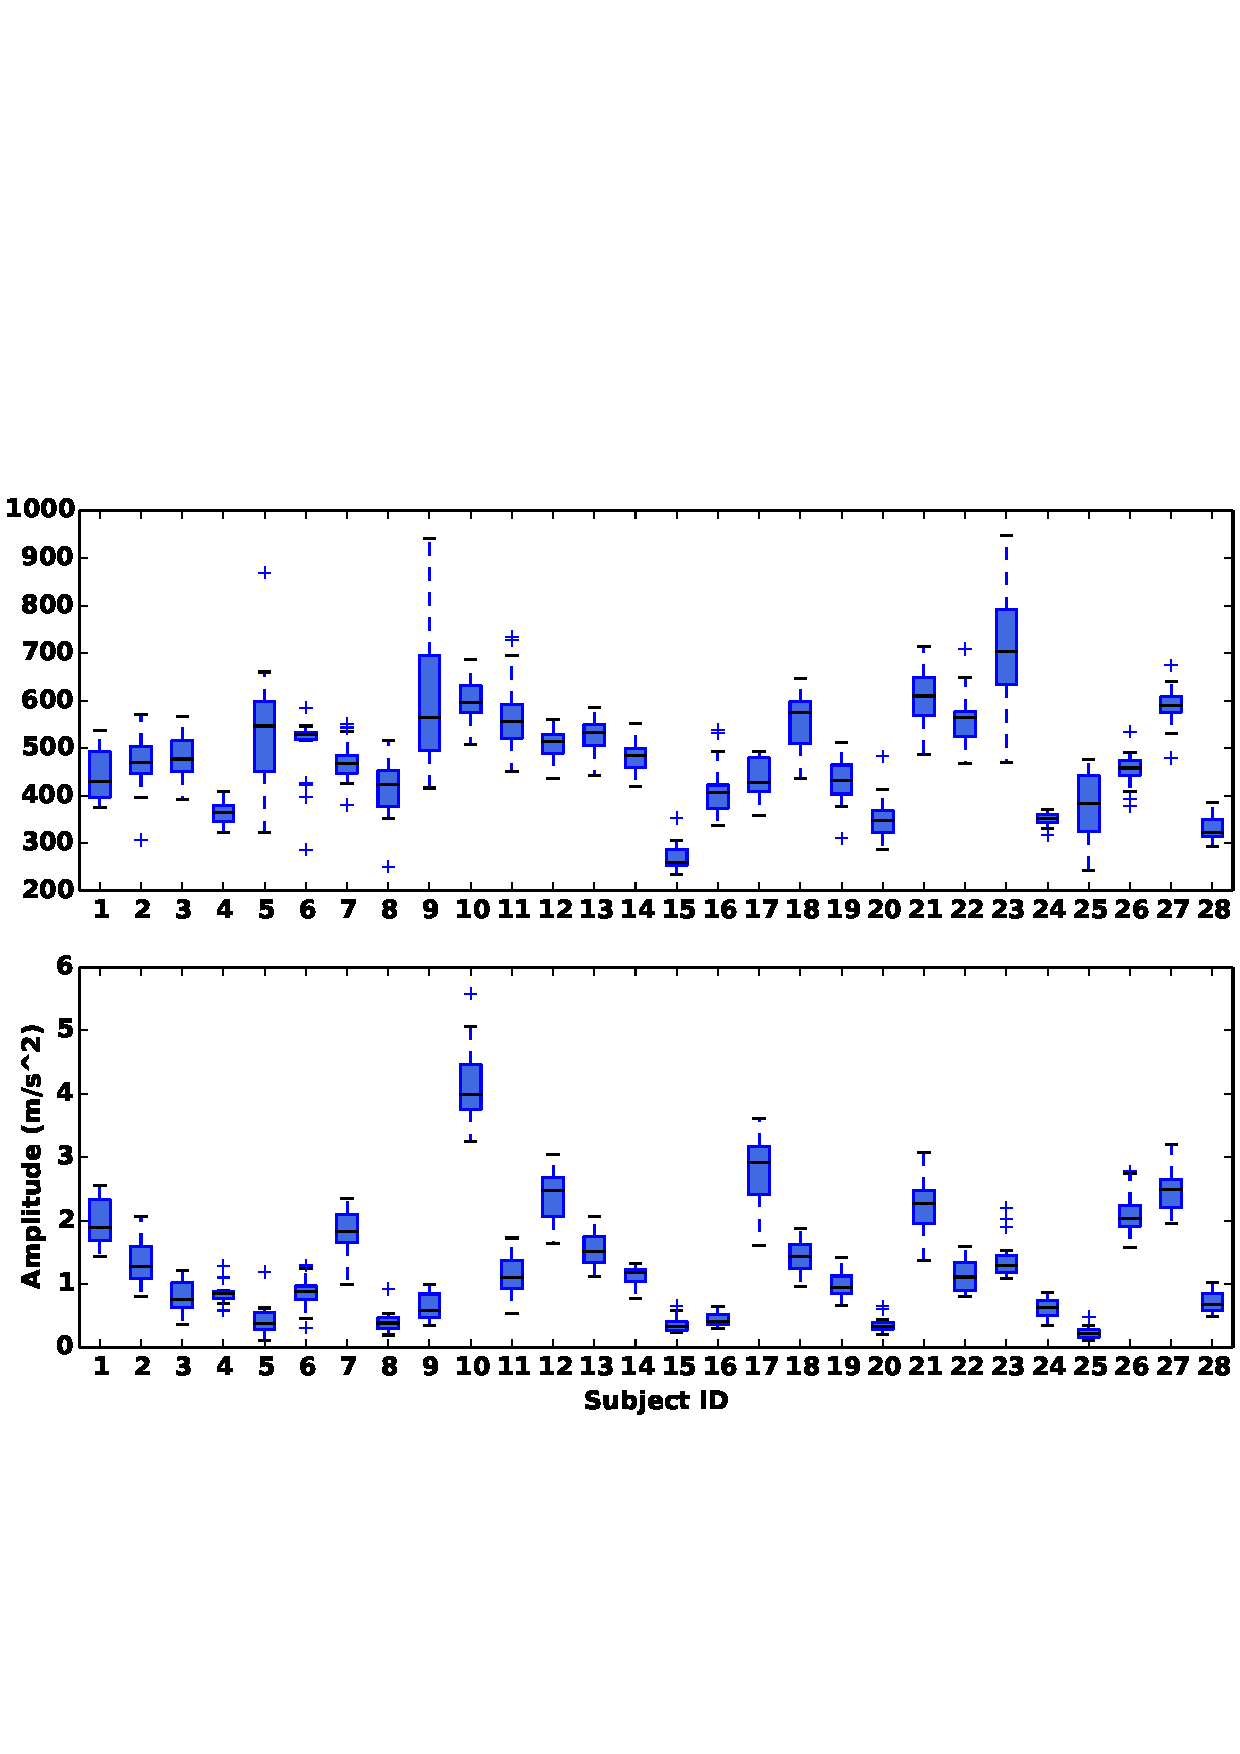
\includegraphics[width=\columnwidth]{figure/width_amp_box.png}
\caption{\label{fig:width_amp} Wave Amplitude and Width Boxplot}
\end{figure}

\begin{figure*}[t]
\begin{center}
\begin{tabular}{ccc}
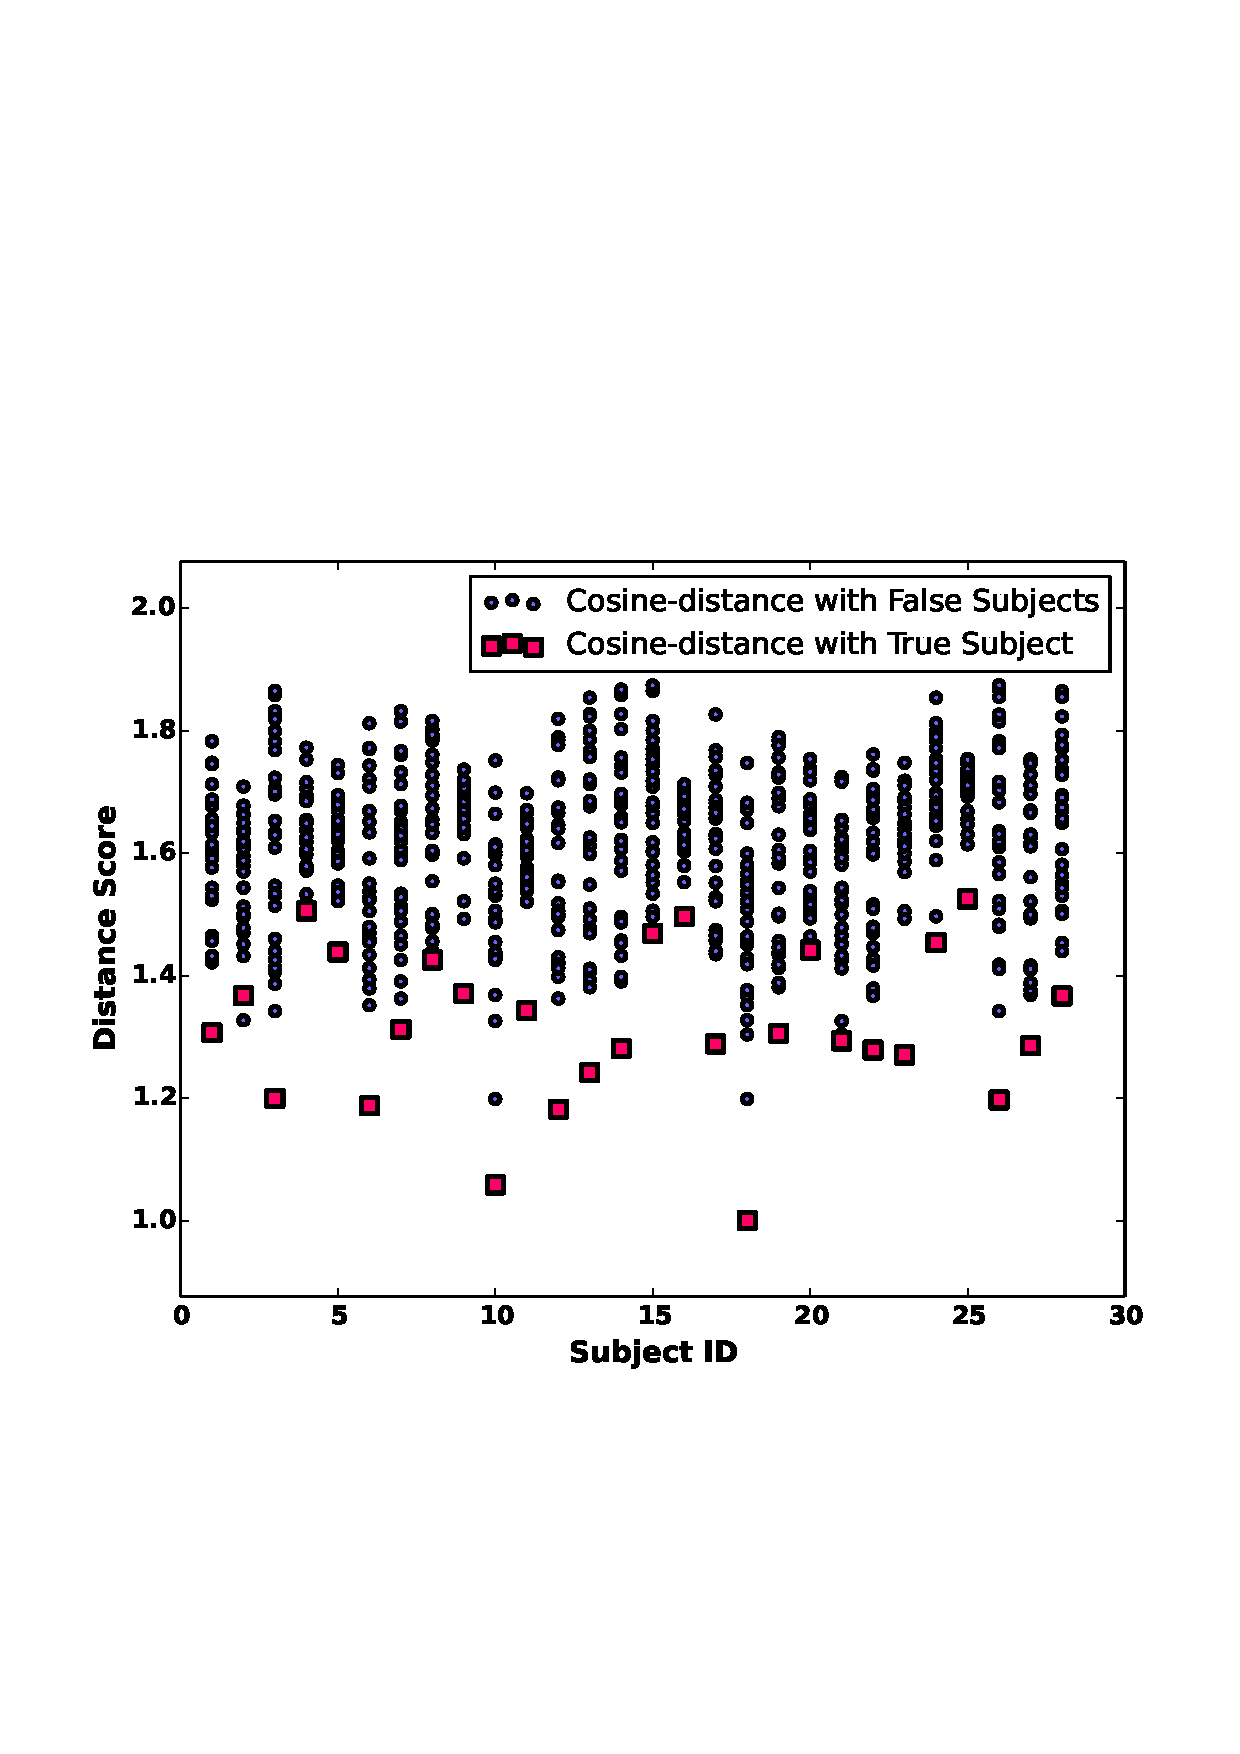
\includegraphics [width=.33\linewidth]{figure/resp_time_cos.png}&
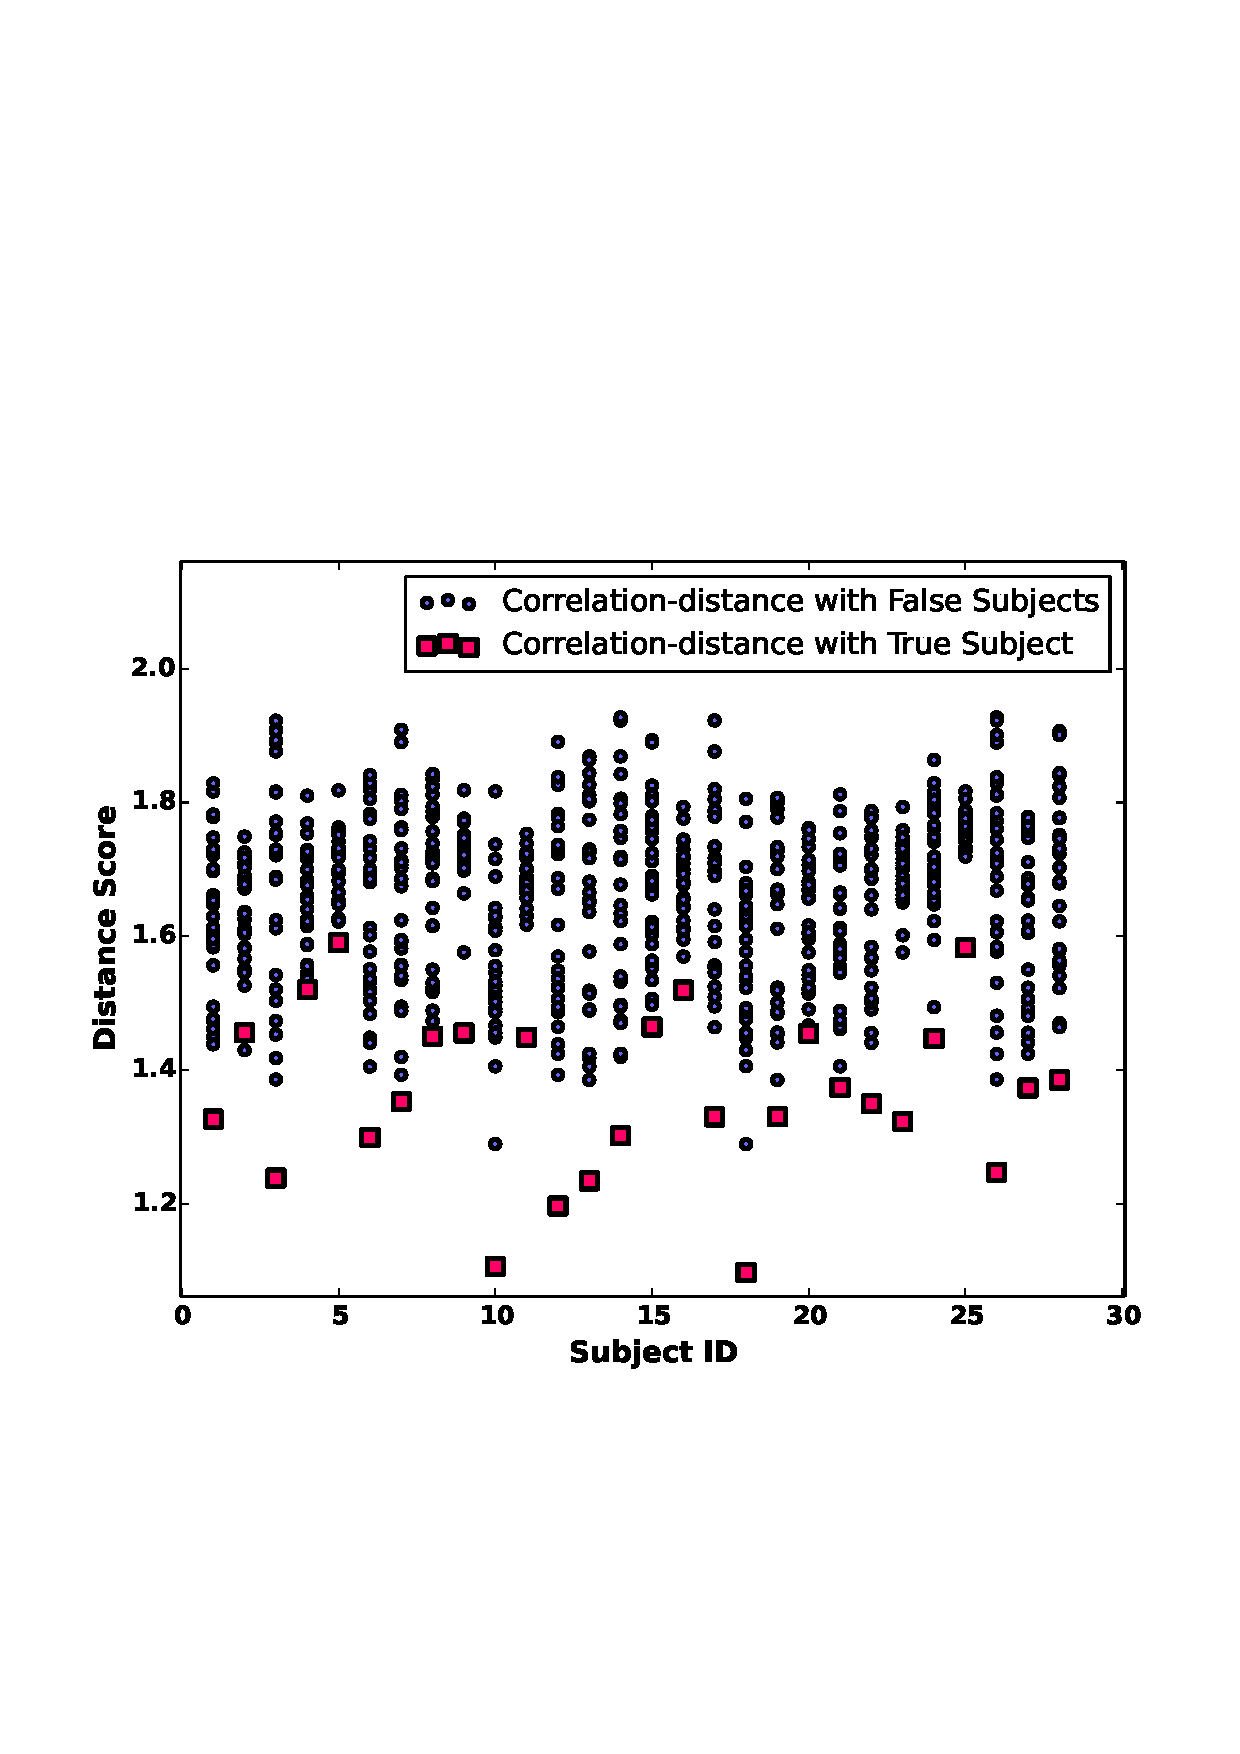
\includegraphics [width=.33\linewidth]{figure/resp_time_cor.png}&
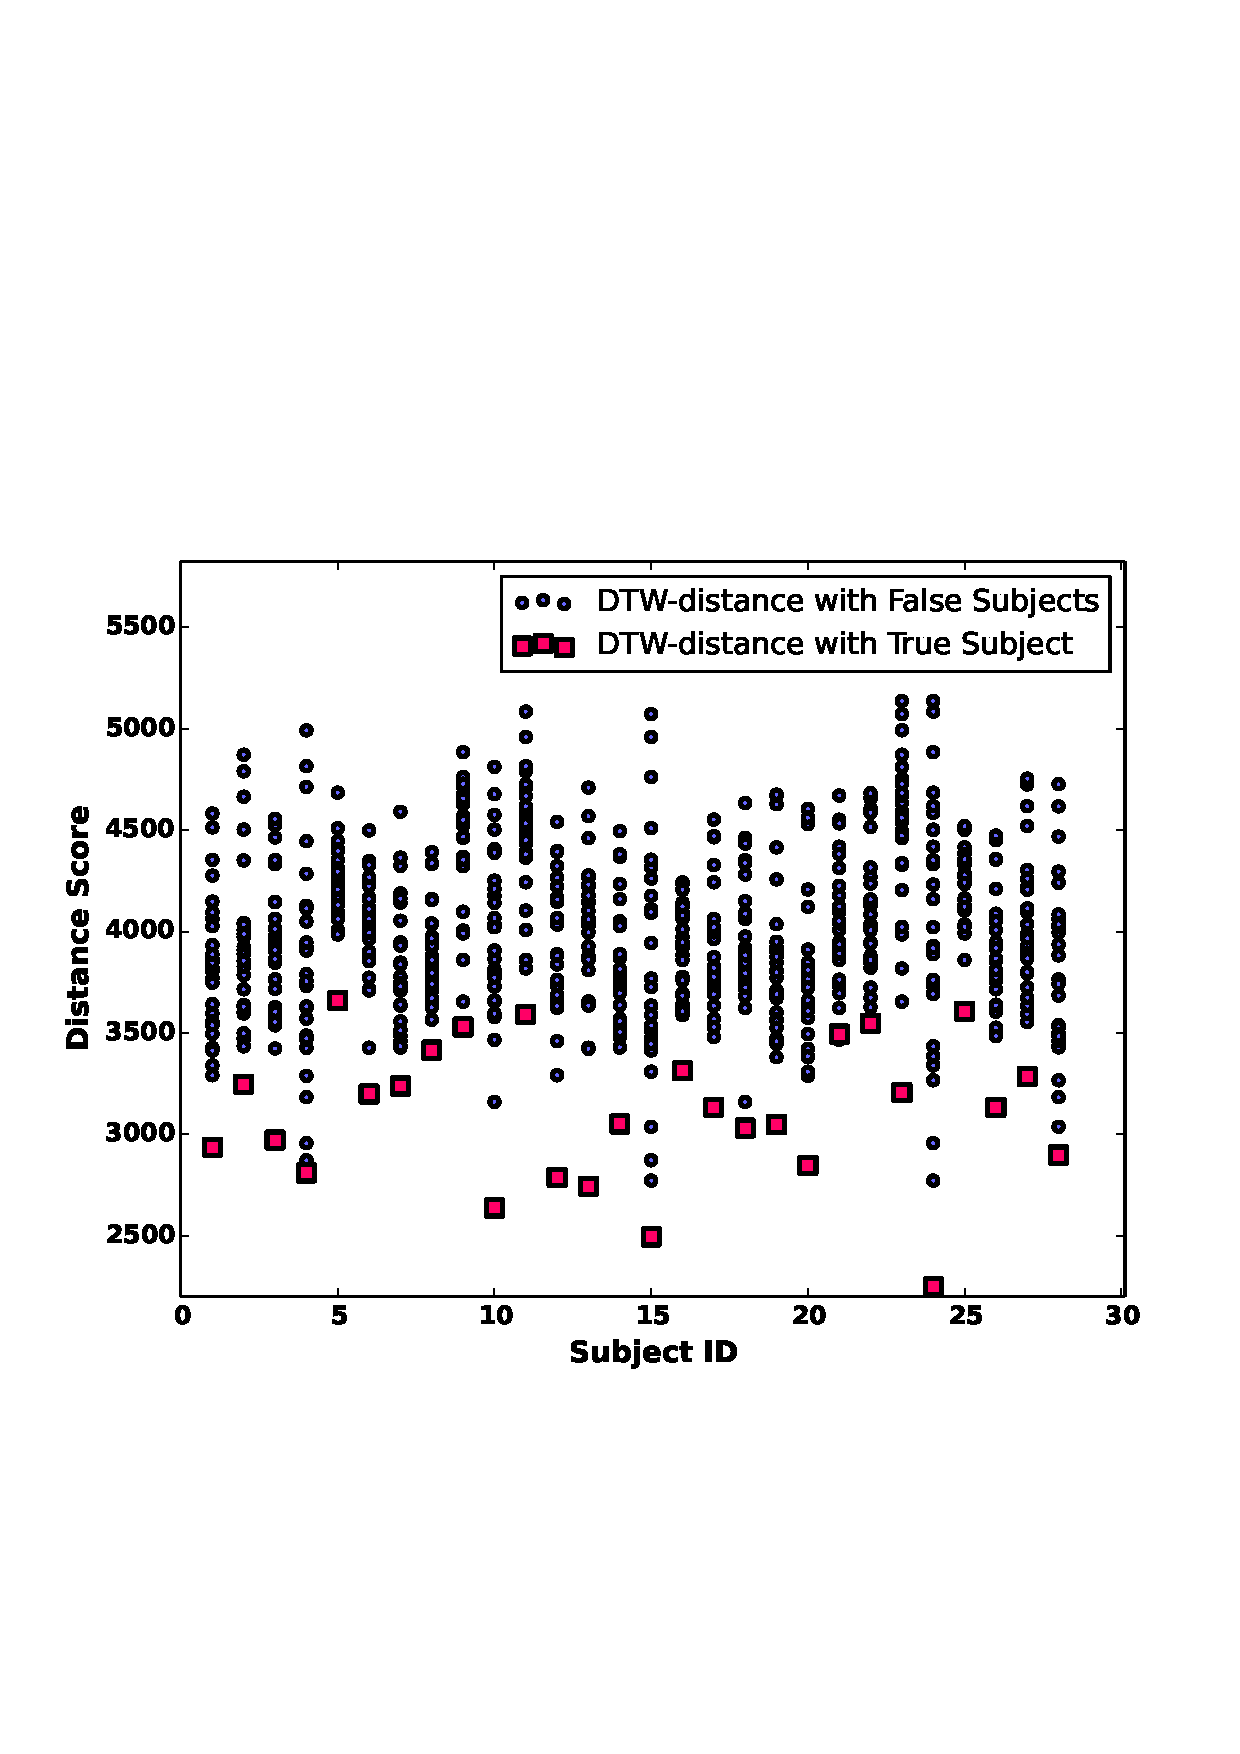
\includegraphics [width=.33\linewidth]{figure/resp_time_dtw.png}\\
(a) Cosine Distance & (b) Correlation & (c) DTW \\
\end{tabular}
\end{center}
\caption{\label{fig:distance} The similarity score is computed over N (N = 20) sample data for each subject, and 28 subjects in total. For each column, a red dot represents the average similarity score of that subject's own SRT, i.e., each of his sample data compared with the other N-1 SRTs from him, hence we have the average similarity score over all these comparison. Similarly, a blue dot on the same column represents the similarity score of that subject's SRTs compares with another subject's SRTs.}
\vspace{-2pt}
\end{figure*}


As shown in Figure~\ref{fig:width_amp}, most of the subject ’s wave amplitude are with different means and small variance compared with their wave width.  To better understand the SRT for different users,  we apply various similarity scores to provide an intuitive and quantitative description of their difference. In Figure~\ref{fig:distance}, the average Cosine Distance (COS) and Correlation (COR) can help most of the subject to differentiate himself with the other subjects, but for some subjects's true subject score (red dot) are closed to their false subject score (blue dot). For subject 2, red dot even exceeds the blue dot.The output of Dynamic Time Warping (DTW)~\cite{cite dtw} can be used as another distance metric.In Figure~\ref{fig:resp_time_dtw},  it shows that all average self-comparing similarity scores are lower than that when they are compared with false users. In real world, the SRT detection algorithm may not be practical if we also consider more complex head-movement other than simple nodding for each beat. The observation above indicates the possibility to further derive a system which can differentiate the true user and the false users based on the fusion of these characteristics.
\section{Headbanger System Design}
\label{sec:design}

\begin{figure}[h]
\centering
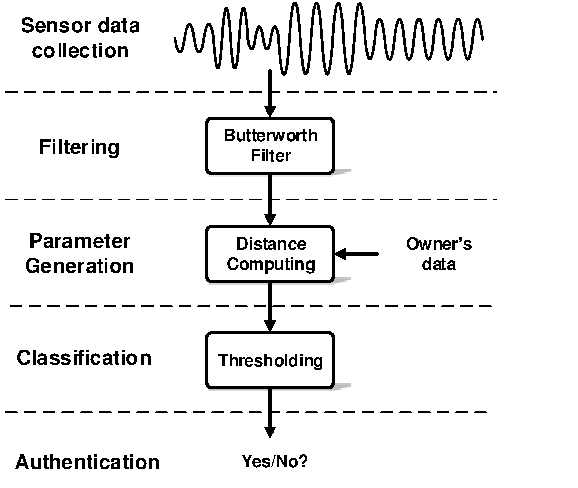
\includegraphics[width=0.95\columnwidth]{figure/system.pdf}
\caption{\systemname~system design flow. The online authentication phase of \systemname~consists of the following steps: (1) sensor data collection in which we collect accelerometer data while users move their head as a response to an audio track played on the glass, (2) filtering in which we apply a Butterworth filtering to smoothen the sensor data for subsequent processing, (3) parameter generation in which we calculate the dynamic time warping (DTW) distances between two accelerometer samples as the parameter, and (4) classification in which we adopt an adaptive thresholding mechanism to classify the user's head movement, whose output will be used as the authentication result.}
\label{fig:sysarch}
\end{figure}

%\begin{figure*}[t]
%\begin{center}
%\begin{tabular}{ccc}
%\includegraphics [width=.33\linewidth]{figure/freq_x.eps}&
%\includegraphics [width=.33\linewidth]{figure/freq_y.eps}&
%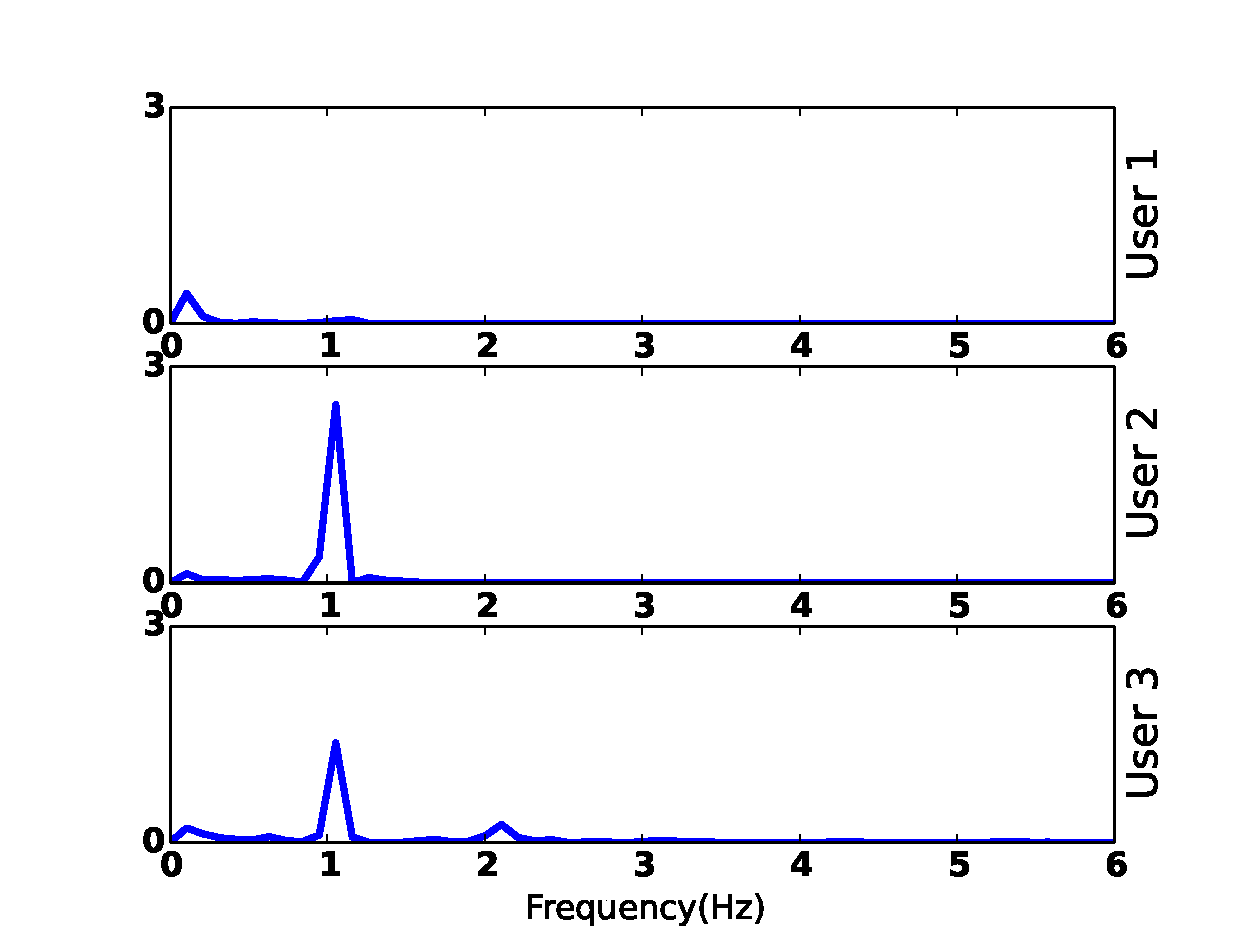
\includegraphics [width=.33\linewidth]{figure/freq_z.eps}\\
%(a) X-Axis & (b) Y-Axis & (c) Z-Axis \\
%\end{tabular}
%\end{center}
%\caption{\label{fig:raw_freq} Accelerometer data from three users, in the frequency
%domain. The data show that the spectrum is significantly
%concentrated within 5Hz for all three users.}
%\end{figure*}

In this work, we design a system, \systemname, that will enable direct authentication of users to their smart-glass device or smart-glass apps using
head-movements.  %We envision that our proposed system will be used as an authentication
%interface on the smart-glass wearable device.
The authentication process has two phases: an offline training phase and an
online authentication phase. In the training phase, the system
collects sensor readings when the real user moves her head with a music cue (following her pre-designed movement pattern), and uses the collected data to
extract the features. We refer to this set of
features extracted through the training process as the {\em trained} dataset
which  serves as the reference in the authentication stage.
In the following discussion, we assume there is only
one real user for the device for the sake of simplicity. An extension to
support multiple users per device will be possible with minor modifications,
namely, by appropriately indexing the users in the trained database.

In the online authentication phase, we collect the sensor readings during a user's authentication attempt, extract features and match them with the trained features.
The user is authenticated upon a successful match.
We posit that \systemname~will run as a service in the device upon power-up or application start-up,
similar to the screen-lock in smartphones.  The authentication process is initiated
by playing a short audio track, to which the user
responds through head-movements. Our design is developed based on the idea that humans respond to music
naturally through head movements, and that such movements are more
significant and unique when the track contains fast beats and/or rhythm.
We will refer to the audio snapshots as {\em music cues} in the rest of the
paper.
%~\systemname~generates unique features from the head
%movements of a user, and uses them as a unique signature for
%identifying the right user of the device. The system will
%grant access only when the head-movement signature
%generated during the login attempt matches with the
%original user's signature.

As illustrated in Figure~\ref{fig:sysarch}, user
authentication in~\systemname~involves the following key modules: sensor data collection and filtering, sample distance computing, classification, and authentication.
%\begin{itemize}
%
%\vspace{-2pt}\item {\em Sensor data collection}: ~\systemname~records the head-movements
%in the form of raw accelerometer signals (in 3 dimensions) using the inbuilt
%accelerometer
%sensor on the smart-glass device.
%\vspace{-2pt}\item {\em Filtering}: The accelerometer signals are filtered by applying
%a low-pass filter to remove records of extraneous motion.
%\vspace{-2pt}\item {\em Parameter generation}: The accelerometer signals are
%processed through the dynamic-time warping (DTW) tool~\cite{dtw} to obtain a
%DTW feature that is treated as the unique signature for the user.
%%A user can generate different signatures for different audio tracks. A
%%training phase collects the set of signature for each user-audio pair.
%\vspace{-2pt}\item {\em Classification}: The signatures are classified as
%a match or not a match, based on a thresholding
%scheme and using the trained data set as a reference. The system grants the
%user access to the device if there is a match
%with sufficient confidence.
%%In the former case, the system will grant the user access
%%\item {\em Authentication}: The head-movement signature generated
%%during system operation is compared with the original user-audio pair
%%signature, and the user is authenticated access if there is a plausible match.
%\end{itemize}
%
%The original signature of the glass user is generated through a
%training phase that is executed when the glass is operated
%by the user for the very first time, and the training data gets
%updated upon each use of the device.
%As shown in Figure~\ref{fig:sysarch} shows the block diagram of
%~\systemname system design.
We will now discuss these design aspects in more detail.
\subsection{Sensor Data Collection and Filtering}
%To facilitate natural head movement, we provide several
%short music tracks with easy-to-follow beats.

The data collection step involves collecting motion sensor data (we mainly focus on accelerometer in this study) while the user makes head-movements
in response to the music cue  with a duration of $T$ seconds.
The raw accelerometer
signals are collected at
a sampling rate of $r$ samples/sec; the default sampling rate on
Google Glass is 50Hz. The accelerometer data corresponding to one user,  is a
collection of accelerometer readings on the
3D axis (x, y, and z) collected over $T$-second duration.
%Figure~\ref{fig:headbanger-illustrate} illustrates the axis
%conventions with respect to the user's head position.
%The data collection unit stores
The accelerometer readings are stored in a
matrix with dimensionality $3\times rT$. %where each element corresponds
%to one signal point.
We will refer to this $3\times rT$ matrix as a {\em sample}.
We retain the duration $T$ to be in the order of few seconds, as frequency of
human head movements are, intuitively, typically in the order of few times per
second. %This intuition will be more clear from the filtering stage to be
%discussed next.
%The sensor data is accumulated in a $30r$ matrix, which we refer to as
%one $ACC$ sample.
%We hypothesize that
%head-movement can serve as a reliable behavioral biometric -- that is, $ACC$
%samples from the same user have smaller distances than samples from different
%users.

%\begin{figure*}
%\begin{center}
%\begin{tabular}{ccc}
%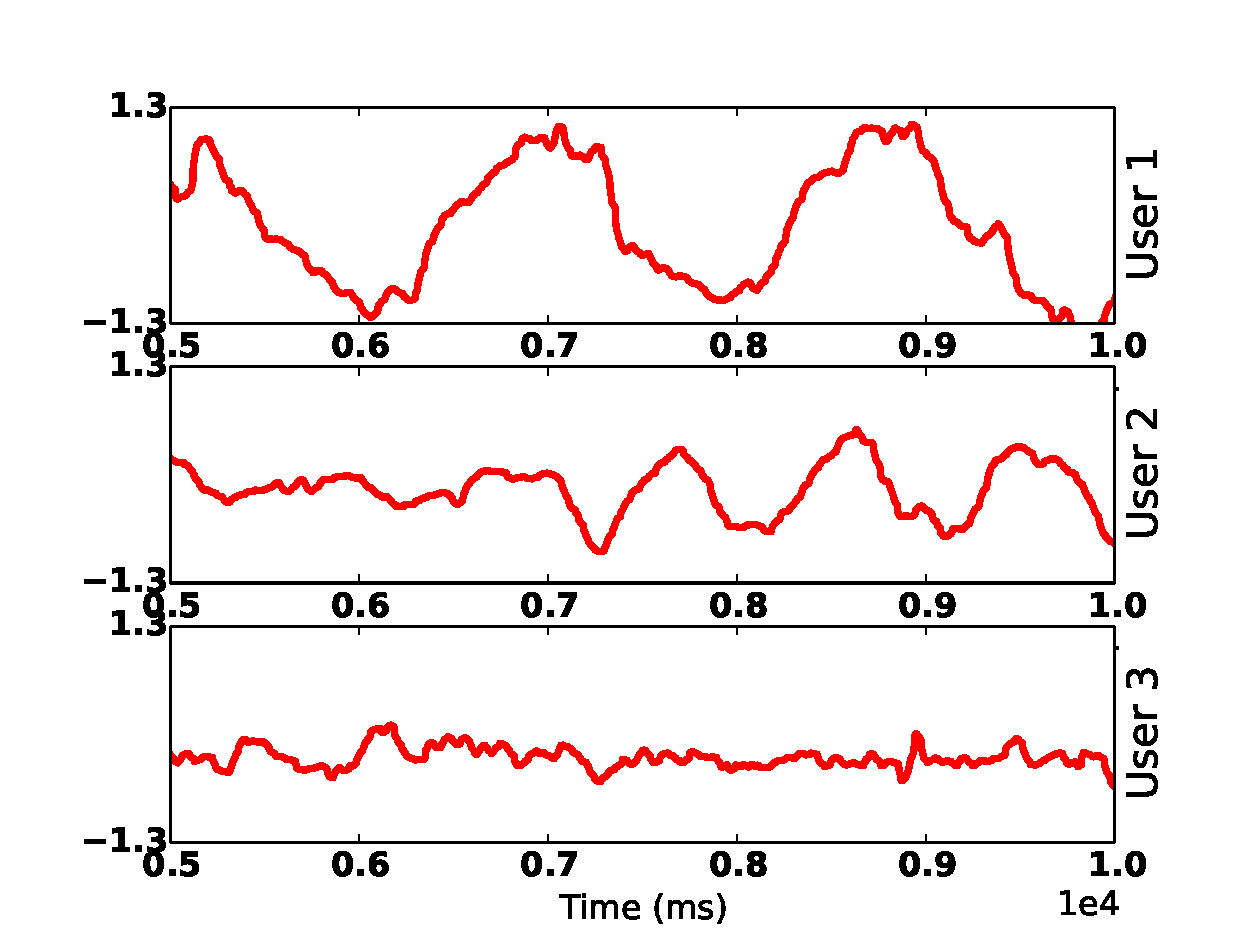
\includegraphics [width=.33\linewidth]{figure/filtered_x.eps}&
%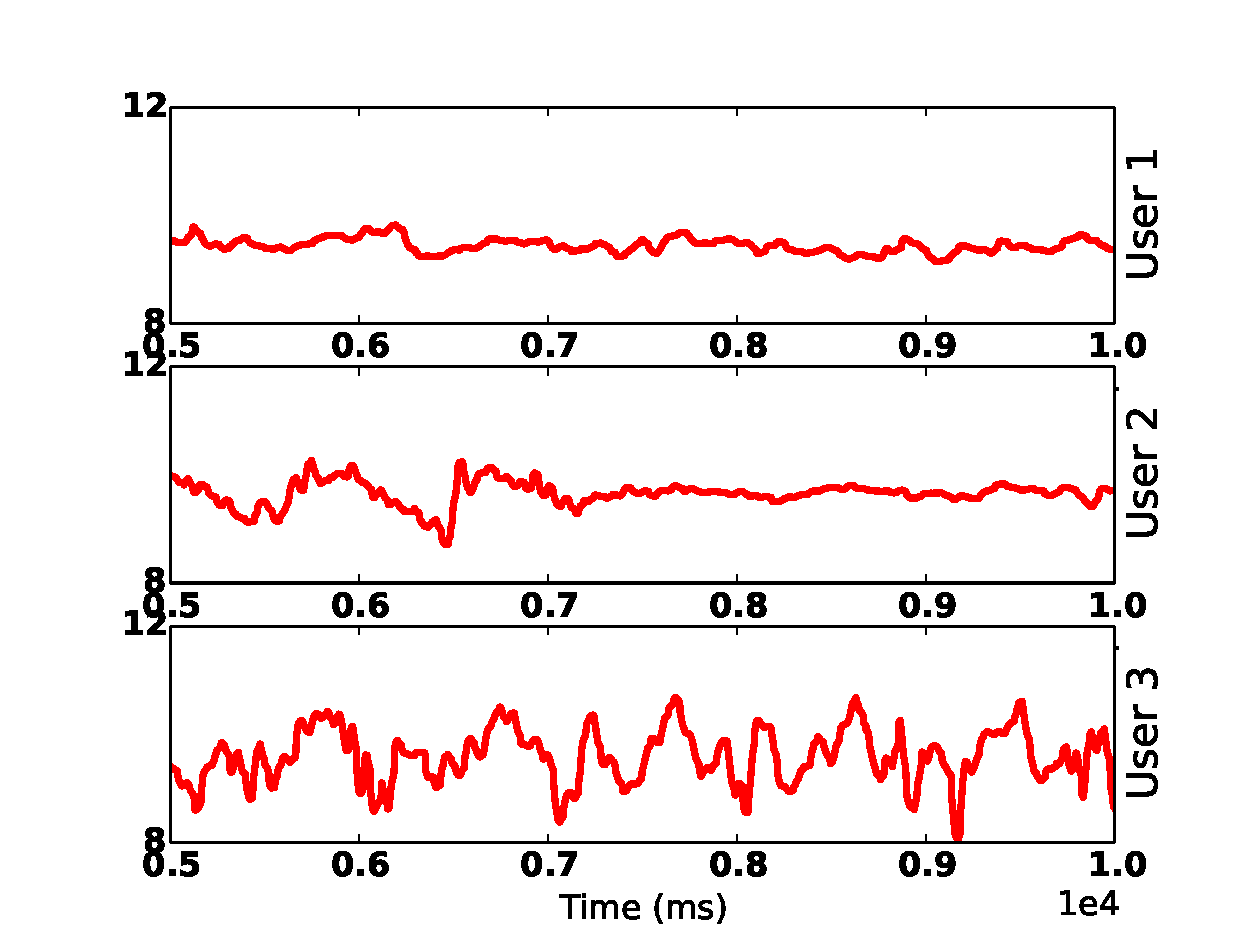
\includegraphics [width=.33\linewidth]{figure/filtered_y.eps}&
%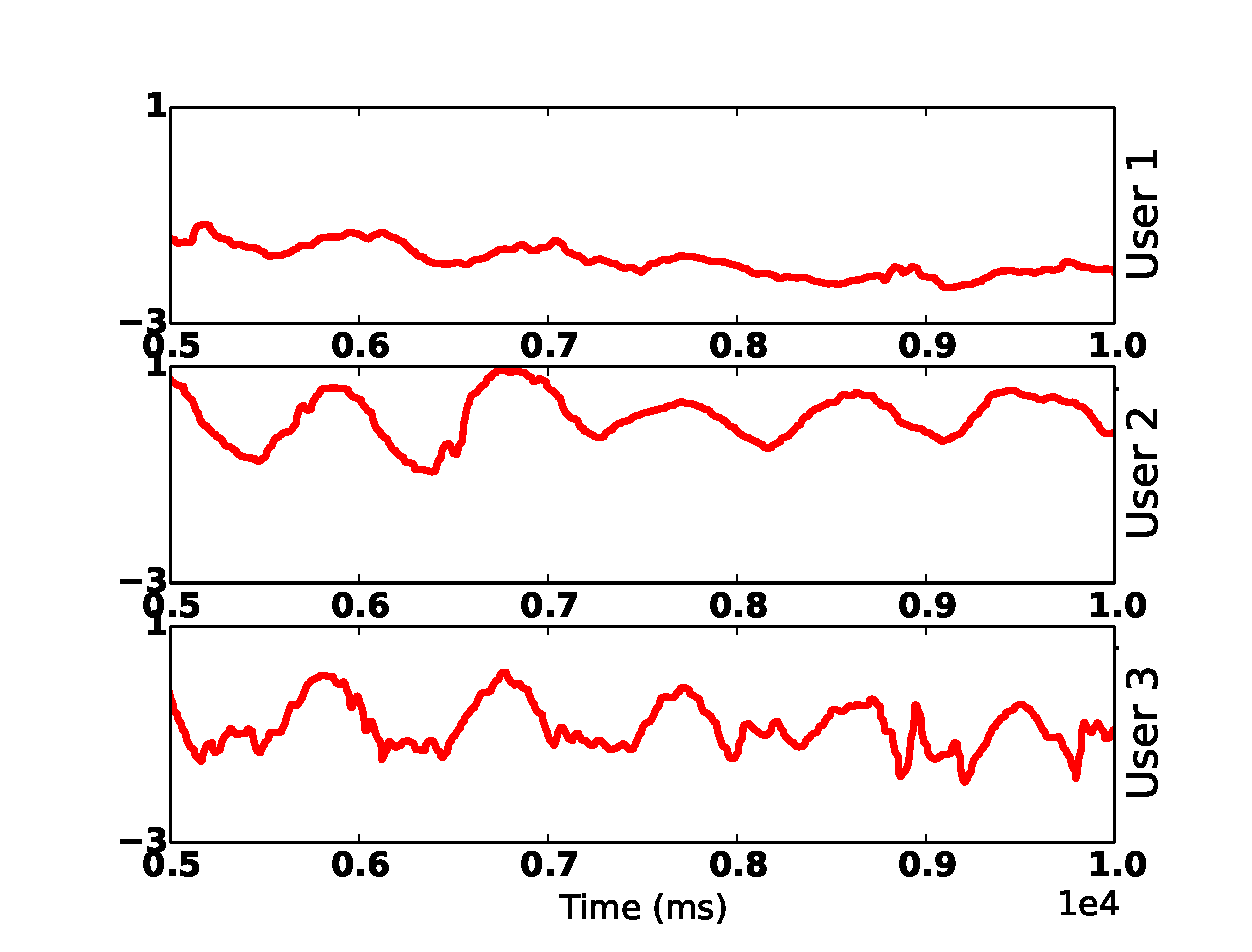
\includegraphics [width=.33\linewidth]{figure/filtered_z.eps}\\
%(a) X-Axis & (b) Y-Axis & (c) Z-Axis \\
%\end{tabular}

%\iffalse
%\begin{tabular}{cc}
%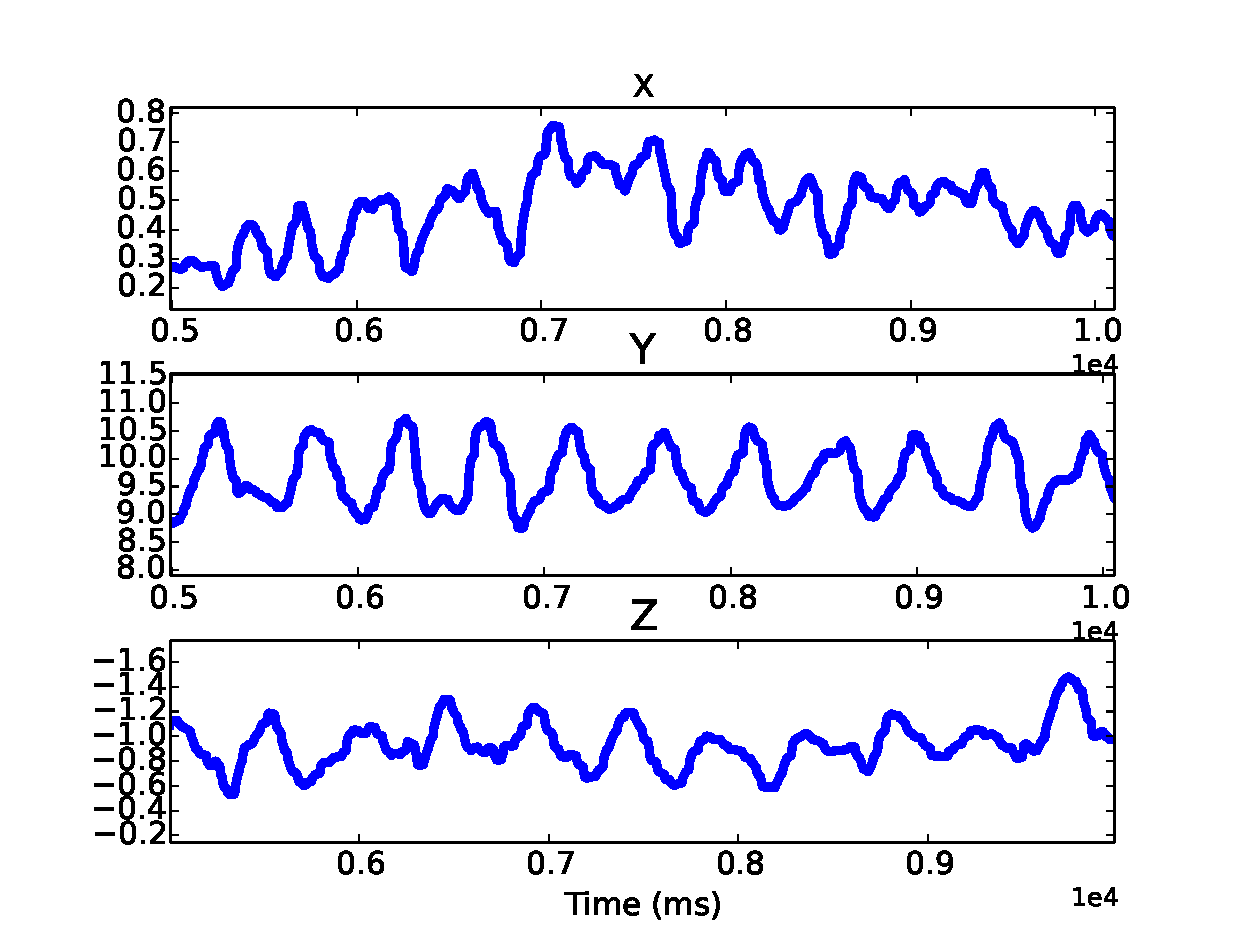
\includegraphics [width=.33\linewidth]{../fig/filer_sub4.eps}&
%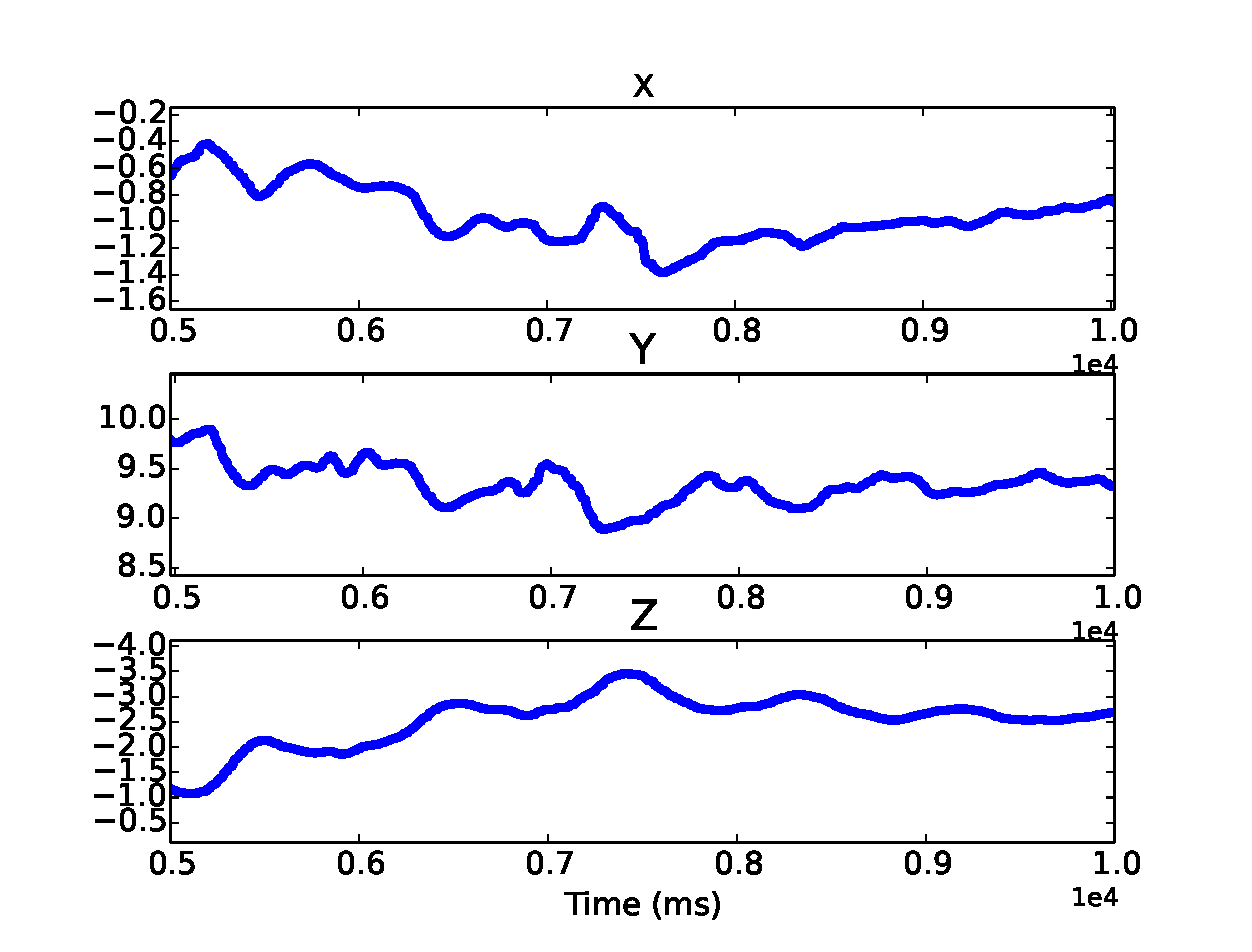
\includegraphics [width=.33\linewidth]{../fig/filer_sub5.eps}\\
%(d) User 4& (e) User 5 \\
%\end{tabular}
%\fi
%\end{center}
%\caption{Filtered accelerometer signals. Applied Butterworth
%filter of order 2 and cut-off frequency 10Hz.
%\label{fig:filteredacc}}
%\end{figure*}


%\subsection{Filtering}

Next, we filter the raw samples to remove noises due to spurious movements such as vibration or shaking.
%The filtering ensures that the head-movement signature
%generated from the accelerometer readings encompasses
%only head movements, and not any spurious signals caused due to
%vibration or shaking.
%From the frequency
%spectrum of each accelerometer sample, as shown in
%Figure~\ref{fig:raw_freq}
%for three users, we can observe that the spectrum is significantly
%concentrated within 5Hz.
%We note that music tracks with high tempo, or fast beats, typically contain
%beats in the order of the order of hundred beats per minute.
%In particular, the high tempo music that we used in our experimentation was
%contained 94 beats per minute~\cite{beats}.
%We infer that the head-movement, in response
%to the beats, will be of the same order. Hence, we hypothesize that
%the signal spectrum in [0,5] Hz range encompass
%human head movements; where 0 Hz can indicate that the head is
%steady still, and 5 Hz can correspond to a vigorous head-shake.
We adopt a low-pass digital Butterworth
filter~\cite{challis1983design} and set a relaxed cut-off frequency of 10Hz.
%Even with the relaxed cut-off, the filtering results in
%clean accelerometer samples with head-movement patterns
%that are prominent and detectable.
%Figures~\ref{fig:filteredacc} (a)-(c) show the filtered results of the raw accelerometer
%samples shown in
%Figure~\ref{fig:raw};
%compared to raw data, the filtered results are much more
%suitable for subsequent processing.

%\begin{figure}[t]
%\centering
%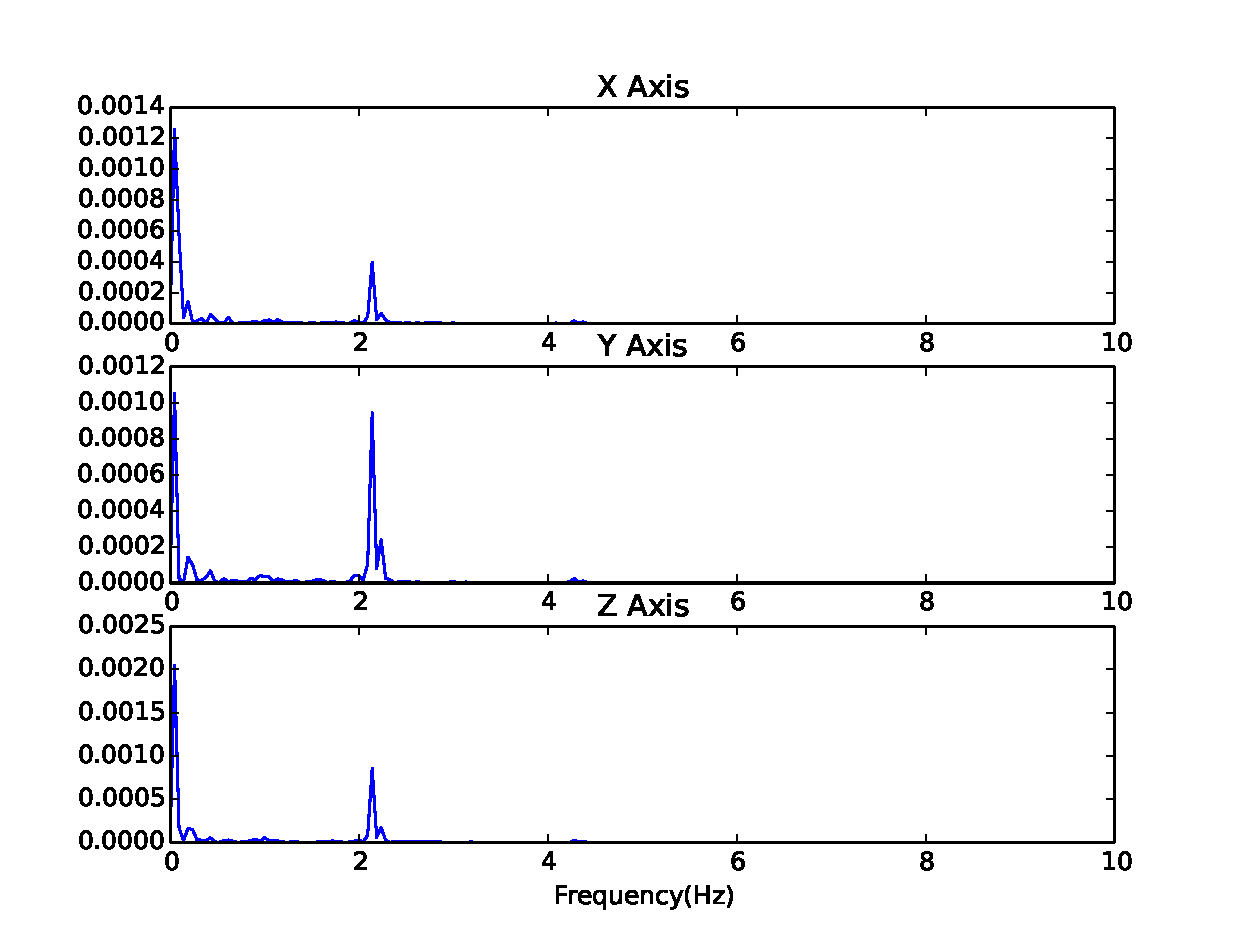
\includegraphics [width=.95\linewidth]{fig/freq_resp.eps}
%\caption{\label{fig:freq_resp}Fiver users' $ACC$ samples in frequency domain.}
%\end{figure}

\subsection{Sample Distance Computing}
%\subsection{Quantifying Sample Similarity}


In this study, we build a distance-based classifier for its simplicity is well suite for wearable devices. There are various ways of computing distances between two signals; we have considered three popular distance-computing algorithms in this study, Cosine Distance, Correlation, and dynamic-time warping (DTW).

Given two signals $s_1 = (x_1, y_1, z_1)$ and $s_2 = (x_2, y_2, z_2)$, its Cosine distance is calculated as***;   Correlation is calculated as ***; DTW is calculated as ***.
%We generate a signature from the accelerometer signals using the
%dynamic-time warping (DTW) tool~\cite{dtw}. DTW is generally used
%as a similarity matching tool for time-domain analysis of
%temporally varying signals.
%DTW compares a temporal signal with a reference (temporal) signal over a
%certain time-window and yields a distance measure as the score. A low score
%(DTW distance) implies that the test signal is in close match with the
%reference.
%We use the DTW to generate a signature for the head-movements
%from the accelerometer signal.
%We observed from our preliminary tests that, users often
%start head movement at an angle with the vertical which varies among users.
%However, we also observed that the head-movements that follow exhibit a
%consistent, and often periodic, patterns over time.
%We empirically observed that the accelerometer signal patterns
%are consistent after the first 1sec duration of head-movements.
%Treating the accelerometer sample set from the first trial as a reference, we
%apply the DTW algorithm on the successive accelerometer sample set to obtain a
%distance score vector, $\hat{d} = (d_x, d_y, d_z)$; the three elements in
%$\hat{d}$ denote the DTW distance score in the $x, y, z$ axes, respectively.
%By computing the mean of the distance scores obtained for each accelerometer
%pair we generate the mean-value DTW distance, which is treated as the
%head-movement signature or unique {\em feature} for that particular user and
%audio
%combination.

%In the offline training phase, we conduct
%%For evaluation purposes, we conduct an elaborate training phase where
%$M$ trials of head-movement exercises, collect $M$ training samples, and
%obtain $M-1$ reference distance vectors. We observed from our evaluations (to
%be discussed in the next section) that $M = 30$ can yield in high accuracy
%while $M = 10$ can yield reasonable accuracy. The trade off is the computation
%overhead that goes into conducting the training (primarily DTW computations)
%for the $M$ samples.
%In real usage of the application,
%the user would conduct only
%two trials of $T$ duration each where trial 1 is treated as reference.
%In this way, the training can be done in-situ. The training data-set is
%updated upon each usage of the authentication interface.
%%Small distance values DTW is expected to return relatively small distance
%%values for samples from the same user, while returning large distance values
%%for samples from different users (that have different movement patterns).
%%Here, $S1$ is the reference

\iffalse
Next we investigate how we can accurately quantify the similarity level
between two accelerometer samples, whose results will be used to classify the users.
After testing various methods,
We decide to adopt the Dynamic Time Warping (DTW) algorithm that is
often used to measure similarity between two waves based on temporal
stimulation.  Unlike many other algorithms, DTW measures the similarity
between two signals that are similar but with phase difference, which is well
suited for our study. In our study, users often start head movement at a
different angle, but exhibit similar, often periodic, pattern for a similar
amount of time. Applying the DTW algorithm on two accelerometer samples $S1, S2$, we
get a vector $(d_x, d_y, d_z)$ denoting the distance in the $x, y, z$ axes
respectively. DTW is expected to return relatively small distance values for
samples from the same user, while returning large distance values for samples
from different users (that have different movement patterns).

YZ: Sugang, we need some detailed equations or algorithms here.
\fi

\subsection{Classification}
The classification step labels a test sample as ``true'' or ``false'' depending upon whether its distance from the real user's training samples is below a threshold. Again, we choose this method because it strikes a good balance between simplicity and performance. Next, we explain how we build the classifier and how to conduct online classification in detail:
%In this study, we developed a simple yet effective classification scheme based on adaptive thresholds.

\begin{enumerate}

\item \emph{Establishing Top-K Samples.} Given $M$ training samples, we first identify the top $K$
samples as follows. For each training sample, we calculate its distances to the rest of the $M-1$ samples, and obtain the average. We choose the $K$ samples that have the lowest average distances and refer to them as Top-K samples.

\item \emph{Calculating True Distance Range.} Suppose sample $s$ is one of the Top-K samples. We have its distance vectors to the rest of $M-1$ samples in the training set, from which we can calculate the mean distance vector $\mu_s$ and standard deviation distance vector $\sigma_s$. Then sample $s$'s true distance range is defined as $[\mu_s-n\sigma_s, \mu_s+n\sigma_s]$, where $n$ is a design parameter that can be tuned. 
    
\item \emph{Labeling Test Sample.}   If a test sample's distance to  one of the Top-K samples, $s$, falls within $s$'s true distance range, it is labeled as a true user; otherwise, a false user. The strictness of this labeling process is characterized by
the value of $n$ in the true distance range; a large $n$ relaxes can increase the false
acceptance rate while a small $n$ value can result in a
high rejection rate of true samples. %In our system we aim to reach an optimal
%value of $n$ that can result in acceptable accuracy.
%\item Steps (1) to (3) are repeated when a new sample set is added to the
%training database resulting in an updated threshold. This way, the thresholding
%based classification is adaptive to the user trials. As we will show in our
%evaluations, the thresholding approach is more robust than the SVM approach,
%through both yield reasonable authentication accuracy.

\item \emph{Voting}. We label the test sample according to all $K$ Top-K samples, and the final classification result is the majority decision among all $K$ labeling decisions. 


%that have
%the lowest $K$ average distance values to the rest of the
%training set. We next calculate their DTW vectors to the rest of the samples in
%the training set to obtain $(M-1)K$ distance vectors. We call this resultant
%vector as Top-$K$ reference distance vector. For example, if $K = 1$, then we
%call the resulting algorithm as Top-1 algorithm; if $K \neq 1$, then we call
%the resulting algorithm as Top-$K$ voting algorithm.
%The voting refers to the procedure that the DTW computation results for each
%sample in the training set is referenced, sorted (in increasing order of DTW
%scores) and the classification (a binary index, match or no-match) is
%performed on the top $K$ entries. The final classification result corresponds
%to the majority vote from the list of $K$ results.
%By using top $K$ samples, instead of all $M$ samples in the training set, we
%significantly reduce the computation overhead in the authentication
%process. In our evaluation, we will study the impact of $K$ value; in
%particular, we evaluate for $K = 1$ and $K = 3$.

\end{enumerate}
Among the four steps outlined above, the first two steps belong to the offline training phase, while the last two steps belong to the online training phase. 
Finally, if the user's test sample is classified as ``true'' then the user is authenticated to the device; otherwise, the user is rejected.


\iffalse
\subsection{Authentication}

The authentication step results in a binary output that corresponds to
either allowing or disallowing the user to unlock the device.
In this paper, we make two reasonable assumptions pertaining to authentication
on the smart-glass device: (i) homogeneity of
accelerometer sensors for all smart-glasses (from a particular vendor), and (ii)
that the device is registered to the user with an associated PIN or passcode,
and that the head-movement signature is used for secondary verification.
Upon entry of the correct password, the device verifies the identity
of the user based on the head-movement signature.

In the head-movement authentication phase, given a test sample, we classify the sample as true (1) or false
(0) based on one of the two classifiers discussed above. If the result is true, the user is accepted; otherwise
the user is rejected.
\fi

%The authentication mechanism for each of the two classification strategies are
%as follows:

%{\bf SVM.} Given a test sample, classify the sample as true (1) or false
%(0) based on the SVM classifier. %If the result is true, compute the euclidean
%distance between the each of the top $K$ true signatures and the classified
%test signature. If the euclidean distance is below a pre-set threshold
%(obtained empirically from training phase)


%{\bf Adaptive thresholding.} Given a testing sample, calculate the
%DTW distance between the testing sample and the top $K$ representative
%samples. If the resulting distance mean falls within threshold range, then the
%result is ALLOW USER; otherwise, the user is rejected. 
\section{Evaluation}\label{sec:results}

%In this section, we will present our evaluation results of the \systemname.
We conducted comprehensive evaluation of \systemname~through laboratory studies involving
human subjects -- our studies were approved by the Institutional Review Board (IRB) of our
institution. In the first phase of evaluation, we collected from volunteer participants accelerometer sensor
readings with Google Glass. We analyzed these traces offline on a PC.
Our evaluations are primarily aimed at determining the accuracy of detecting
and differentiating users based on their head-movements, and understanding
the effect of important parameters such as similarity metric, length of the music cue, training
data-set size and sampling rate. In addition to authentication accuracy, we also evaluated how robust is \systemname~against intentional imitation.
In the second phase of evaluation, We also measured the response time of our Google
Glass implementation of \systemname.

%based on profiling the execution time of each key
%functions associated with \systemname, on the Google Glass device.

\begin{figure}
\includegraphics[width=\columnwidth]{figure/roc_dtw_cos_cor.png}
\caption{\label{fig:roc_dtw_cos_cor} The impact of the distance computing algorithm (i.e., DTW, cosine distance, and Correlation). In this set of results, we varied the value of $n$ from 0.0 to 10.0 with an increment of 0.1, resulting in 100 data points in each case. We then plotted the TPR (y-axis) and FAR (x-axis) for each data point. Our results show that DTW delivers much better accuracies than the other two distance algorithms.}
\end{figure}

\begin{figure}[t]
\centering
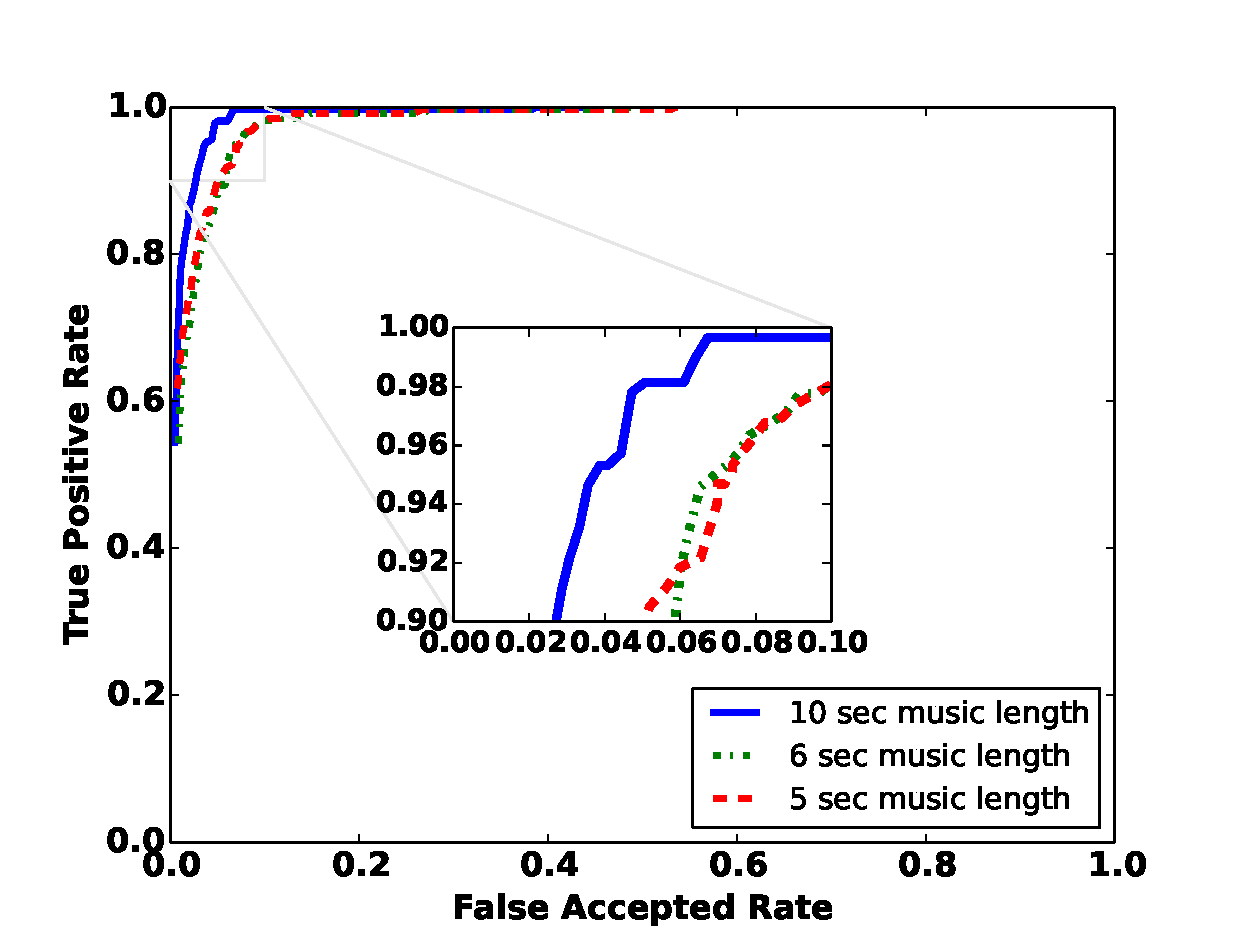
\includegraphics [width=\columnwidth]{figure/top1_roc.eps}
\caption{The impact of music cue duration on TPR and FAR in Top-1 scheme ($K = 1$). We trimmed a 10s music snapshot into music cues of 10s, 6s and 5s correspondingly. In this set of results, we varied $n$ ***YZ: what is n? What are the values n? Please specify ***}
%The variable here is $n$. Each (TPR, FAR) data point in the curve corresponds to a different value of $n$}
\label{fig:roc-top1}
\end{figure}

\begin{figure}[t]
\centering
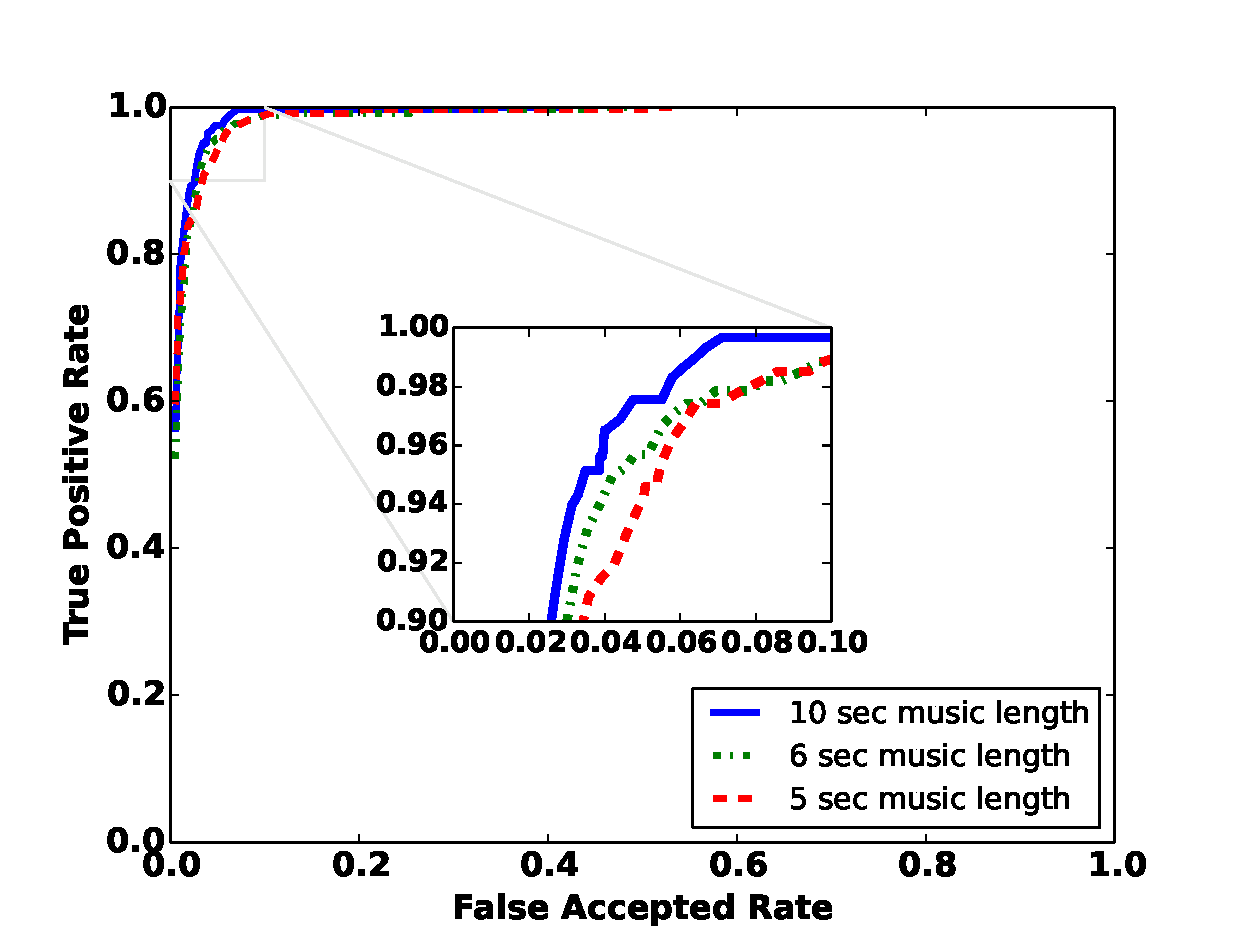
\includegraphics [width=\columnwidth]{figure/top3_roc.eps}
\caption{Evaluation of impact of music cue duration on TPR and FAR in Top-3
voting scheme ($K = 3$). A 10 sec music snapshot is trimmed into music cues of
10 sec, 6 sec and 5 sec correspondingly.The variable here is $n$. Each (TPR, FAR) data point in the curve corresponds to a different value of $n$}
\label{fig:roc-top3}
\end{figure}

\begin{figure}[t]
\centering
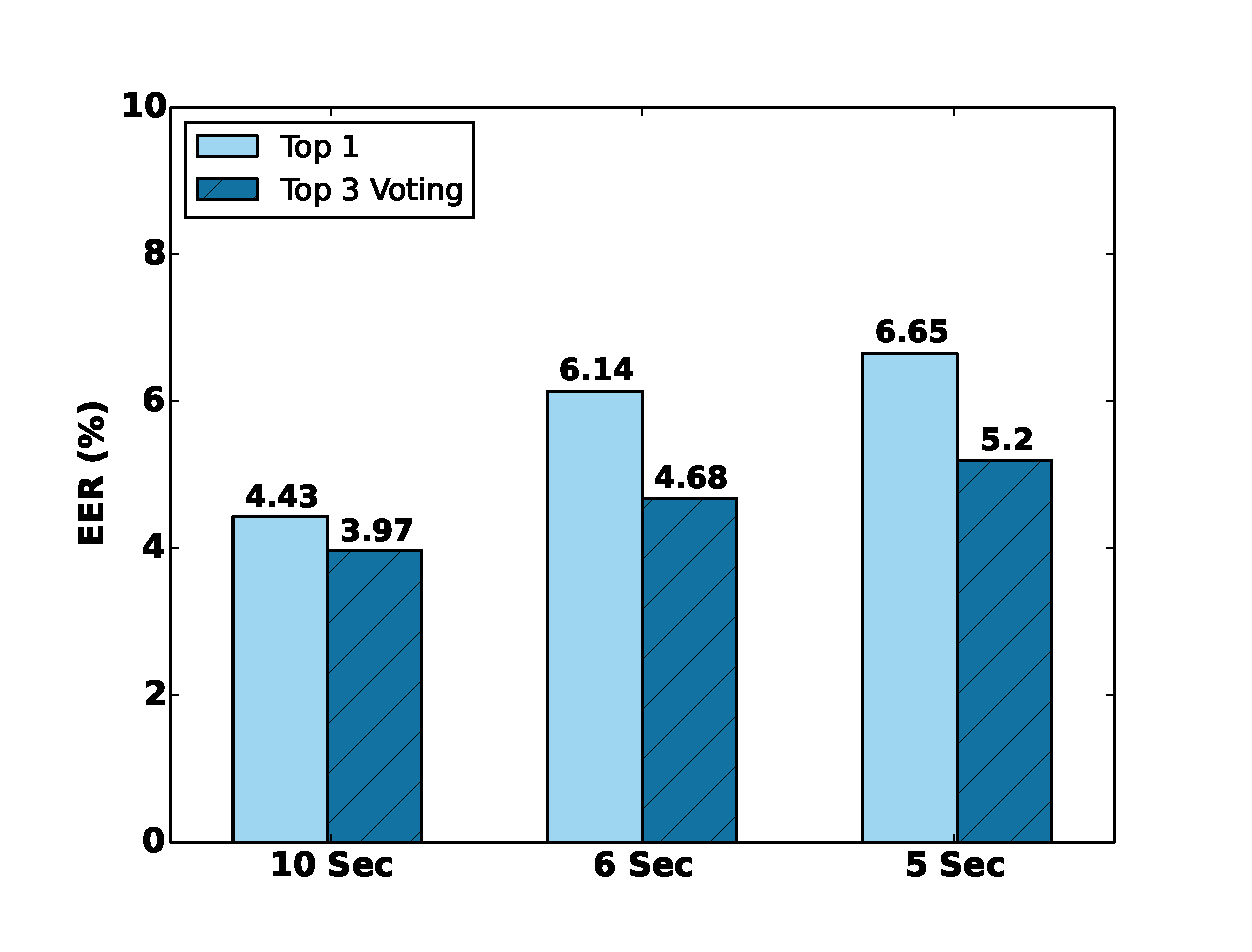
\includegraphics [width=\columnwidth]{figure/exp2_vary_length.eps}
\caption{Comparison of EER for different music lengths (10 sec, 6 sec and 5
sec) with a fixed n value of 2.7}
\label{fig:eer-length}
\end{figure}



\begin{figure}
\includegraphics[width=\columnwidth]{figure/roc_dtw_diff_freq.png}
\caption{\label{fig:roc_dtw_diff_freq} Evaluation of impact of different sampling rate shows that the highest sampling rate 200 Hz gives the best resutlt. However, the sampling rate determines computational effort for the smart device, which could be significant in terms of response time.}
\end{figure}


\subsection{Authentication Accuracy of \systemname}

\subsubsection{Participants}
We had a total of 30 volunteer participants for this experiment, including a total of 19 males and 11 females.
The average age of the participants was 29.7 years with a standard deviation
of 9.81 years. The youngest participant was 23 years old while the eldest was
54 years old.

\subsubsection{Procedure}
Our first experiment setup aimed at emulating the typical usage scenario
of \systemname~for authentication, where a user conducts head-movements in
response to a music cue played on the Google Glass device during a login
attempt.
%One of the participants executing the experiment trial wearing the
%Google Glass. %Figure~\ref{fig:setup} shows our experiment setup.
In this experiment, all participants were asked to wear a Google Glass
device. Participants who originally wore spectacles were asked to remove their
spectacles before conducting the experiment.
The trials were conducted in an academic environment and overseen by one of
our team members.
The Google Glass ran our data-collection app that played a piece of
music (music cue) for a specific duration, and recorded the accelerometer
sensor readings. We conducted these trials for three duration values: 5s,
6s and 10s. %As we will show further, the accuracy of the system can
%significantly improve with the duration of the music cue; longer the duration
%better is the accuracy.
The sensor readings were recorded into a text file that was stored
in the Glass's memory and later transported to a PC for offline processing
through a Python script. The experiment was conducted in a well-lit indoor
academic laboratory environment.

During the course of a data collection session, the participants were allowed to take a
break or withdraw from data collection if they felt uncomfortable at any
point; for example, feeling
dizzy after head-movement for a period of time, not being able to see clearly
if near-sighted, etcetera. The conductor also allowed the user to take a break
of about one minute after each trial.
Each trial lasted for the duration of the music cue played on the Glass, and
a total of 40 such trials were conducted for each of the 30 subjects.
The entire data collection effort lasted over a duration of 60 days, of which 15
subjects conducted their trials in a single sitting over a period of two
hours, while the rest of the trails were spread over 3 days on an average per
subject.
%while, half of the trials of the rest 10 subjects were spread over 2 days.
The experiment yielded three sets of data traces that each correspond to
the three music cue durations we selected.

\subsubsection{Metrics}
We evaluate the accuracy of \systemname~using metrics that are commonly used
in evaluating authentication systems, namely,
true positive rate TPR (percentage of true test samples that are
correctly accepted), false acceptance rate FAR (percentage of false test samples that are
mistakenly accepted), and false rejection rate FRR (percentage of true test
samples that are mistakenly rejected). These three metrics are, however, largely dependent on the choice of thresholding values in the system design --
a strict threshold in the classifier can lead to high FRR, while
overly relaxing the same can lead to a high FAR. Hence, in order to report the threshold-independent, end-to-end performance, we consider
the equal error rate EER (percentage of errors when $FAR = FRR$), that
considers both FAR and FRR. ***YZ: please check whether this is correct ***
%%and balanced accuracy BAC, where BAC = 1 - (FAR+FRR)/2.
%%We present the accuracy results through the receiver operating
%%characteristics (ROC) curves, TPR versus FAR, as shown in Figures~\ref{}
%%and~\ref{}.
%Figures~\ref{fig:roc-top1}, \ref{fig:roc-top3} and \ref{fig:eer-length} report
%the accuracy
%of \systemname~through the metrics stated above.
%%Figures~\ref{fig:roc-curves} (a)-(c) report the accuracy of
%%\systemname~through the metrics stated above.

%In general, we observe that even with a 5s music cue, \systemname~can achieve a TPR of ***\% at FAR of ***\% and EER of ***\% (when we have $K$=***, *** out of 40 trials from each user being used for training with  thresholding parameter value $n = 2.7$ with DTW). If users do not mind a cue duration of 10s,

%After evaluating the above metrics under various scenarios, the highlight is that \emph{our TPR can be as high as 95.1\% at FAR of 3.5\% and EER of 3.97\%} (when we have $K = 3$, and 30 (out of 40) trials from each user being used for training with a thresholding parameter value $n = 2.7$ with DTW). Next we discuss in more detail how the authentication accuracy results are impacted by various design parameters.

\subsubsection{Determining System Parameter Values}
Before presenting the final authentication accuracy results, we first report how \systemname~TPR and FAR are impacted by several important system parameters, namely, the choice of distance computing algorithm, $K$ value, and training dataset size, in Figures~\ref{fig:roc_dtw_cos_cor}, ***, and *** respectively, and determine the values we are going to use for these parameters. In each set of results, we varied the value of $n$ from 0.0 to 10.0 with an increment of 0.1, and had a total of 100 data points. We then plotted the TPR (y-axis) and FAR (x-axis) for each data point, and the resulting curves are referred to as ROC curves ***YZ: more details about ROC *** In this setting, between two ROC curves on the same figure, the one that is closer to the upper left corner of the figure yields better authentication accuracy.

Firstly, Figure~\ref{fig:roc_dtw_cos_cor} compares the performance of three distance computing algorithms: DTW, Cosine Distance, and Correlation in this study, when we had $K=***$, music cue duration of 10s, and training dataset size of 30 samples.  Among these three algorithms, DTW fares much better than the other two: DTW is ***\% better than Cosine Distance, and ***\% better than Correlation. This is as expected because DTW ***~\cite{DTW}. As a result, in the remaining of this study, we will use DTW for the end-to-end system design. 

Secondly, Figure~\ref{fig:***} compares the performance of two $K$ values: $K$=1 and $K$=3, when we had DTW, music cue duration of 10s, and training dataset size of 30 samples.  Recall that the classification algorithm in ~\systemname~generates a classification result (YES or NO) by voting among individual results each generated by the top-K samples in the true set. Hence, we expect that considering top 3 samples will be better than only considering the top 1 sample, as confirmed by the results shown in Figure~\ref{fig:***}. However, we observe the improvement is only marginal: the accuracy when $K=3$ is only ***\% better than the accuracy when $K=1$. On the other hand, having $K=3$ incurs three times as much computing as having $K=1$. As a result, in the remaining of this study, we will use $K=1$ for the end-to-end system design.

Thirdly, Figure~\ref{fig:***} compares the performance of three training dataset sizes: 10, 20, and 30 samples, when we had DTW, $K=1$, and music cue duration of 10s. We observe that ***. As a result, in the remaining of this study, we will use *** for the end-to-end system design.

%\paragraph{Impact of Training Dataset Size}
%%The accuracy of detecting and matching the head-movements to the user depend
%%upon the music cue duration, value of $K$, and number of samples used for
%%training.

%***YZ: we need to rewrite this section. In this section, we need to focus on how much improvement we have when we increase the data set size. Also, I think we are using way too many metrics. ***
%Recalling from Section~\ref{sec:design}, the input to the training phase
%is a set of temporal signals (samples with duration equal to the music cue
%duration), each corresponding to one trial of the head-movements from the
%user. Our evaluations so far considered a training set consisting of 30 samples.
%***I feel we have too many different metrics. It is confusing.*** In Figure~\ref{fig:eer-size}, we report the EER in \systemname~for three
%different training data set sizes; 10,20 and 30 samples.
%We can observe from Figure~\ref{fig:eer-size} that the EER holds an inverse
%relationship with the training set size. A larger training set minimizes the
%variance in mean and standard deviation computations, as the errors in their
%inconsistency are reduced by averaging the mean and standard deviation
%estimates over a larger set of data.
%On the other hand, a larger training set also implies a longer execution time
%of the training phase.
%However, in our system design, we posit that the training phase can be
%conducted
%offline on a more compute efficient device (smartphone, PC or server) and that
%the wearable device can pre-fetch the trained data (for example, an XML file),
%prior-to or during data collection phase, through a wireless link.

%are giving promising results for the response time sequence, hence we will evaluate these three algorithms in our end-to-end system. Also due to DTW is relatively more computing-intensive than the other two algorithm, we would like to see whether DTW  is worth of computing resource. In this experiment, we vary thresholding parameter value $n$ and fix the other parameters: 10 sec duration, $K = 1$, and  training data $size = 30$. We can observe from the ROC
%(receiver operating characteristic) curves in Figure~\ref{fig:roc_dtw_cos_cor} that DTW gives the best result among three algorithms, since its curve is the closest to the upper left corner. Our system preserves all characteristics of the data, which includes the response time to the music beat and the 3-axis accelerometer data. In terms of matching the waveform of two signal, DTW can achieve significant enhancement than the other two algorithms~\cite{DTW}.

%\paragraph{Impact of $K$ value}
% We observe from the ROC curves in Figure~\ref{fig:roc-top1} and \ref{fig:roc-top3} that
%for both, $K=1$ and $K=3$, the TPR is close to 95\% while the FAR is slightly
%above 3\% for the 10 sec music duration. For $K = 1$ the FAR increases to
%about 7\% for the 5 sec and 6 sec cases, however, for $K = 3$ the FAR
%decreases to about 3\% and 4\%, respectively.
%We observe a similar trend with the EER as shown in
%Figure\ref{fig:eer-length}, where improvements of 0.5 - 1 \%
%can be achieved by choosing $K = 3$ over $K = 1$. ***YZ: if the improvement is less than 1\%, then K=1 is sufficient. Then for the music cue, please just use K=1***
%This indicates that the accuracy in \systemname~can improve with a larger
%value of $K$. However, the improvement in accuracy through redundancy in the
%training set trades off with the increased execution time as the
%matching requires at least $K - 1$  extra DTW computations as opposed to only
%1 for a top-1 scheme. As we will show ahead, DTW computations incur heavy CPU
%budget on the wearable device.
%***YZ: I will re-write this paragraph after you reorganize the results ***



\subsubsection{Authentication Accuracy Results}
%We measure the DTW computation on Google Glass to be the most
%computationally expensive operation of all the software modules in
%\systemname.
%\paragraph{Impact of music cue duration}

%***YZ: I need to rewrite this paragraph. The tone needs to be changed. What is the improvement? ***

After determining the system parameters' values for~\systemname~, we next report the EER of~\systemname~when the user chooses different music cue durations in Figure~\ref{***}. After a user starts the authentication procedure, how long a user must wait before she receives the authentication result is an important quality-of-service metric, which we refer to as \emph{authentication latency}.  The authentication latency consists of two parts: data input latency and computing latency, where the former is the time a user spends on listening to the music cue and making head movements while the latter is the time \systemname~spends on computing the authentication result. Between these two parts, the data input latency is the bottleneck as the computing latency can be easily reduced (by better algorithms and/or faster hardware) and/or hidden (by pipelining computing with data collection). Unfortunately, the data input latency is hard to be reduced or hidden by the improvement in software or hardware. Recognizing that different users can tolerate different data collection latencies as well as desire different levels of authentication accuracies, \systemname~allows the users to choose different music cue durations (which has the same length as the data input latency) and delivers different authentication accuracies accordingly.

From Figure~\ref{fig:***}, we observe that the EER is as low as *\% with a 5-second music cue, and ***\% with a 10-second music cue.  
%
%In general, we observe from the results that the FAR can
%be decreased by increasing the music cue duration.
%We can observe (from Figures~\ref{fig:roc-top1}, \ref{fig:roc-top3} and
%\ref{fig:eer-length}) that the improvement is less significant when the music
%cue duration is increased from 5 sec to 6 sec, however, the improvement is
%more
%significant when the music cue duration is increased to 10 sec.
%In \systemname~the data collection phase for the authentication system
%(sampling accelerometer sensor readings) is executed in parallel with the
%music cue. The data processing phase involving the filtering, classification
%and matching is executed only at the end of the music cue and in the same
%order.
%Hence, execution time of the app will be independent of this duration.
We note that, the data input duration of 5-10 sec for authentication is on par with those
of password based systems~\cite{von2013patterns}, *** details**.
%We also note that, since the authentication process is initiated only at the
%end of the music cue, execution time of the app will be independent
%of this duration.

\begin{figure}[t]
\centering
\includegraphics [width=\columnwidth]{figure/exp2_vary_size.eps}
\caption{Comparison of EER for different training sample sizes (30, 20 and 10)
with fixed n value of 2.7}
\label{fig:eer-size}
\end{figure}





%\paragraph{Impact of Sampling Rate}
%***YZ: this can be removed ***
%Due to DTW is resource-consuming, one direct way to reduce the workload of our algorithm is to decrease the sampling rate of the accelarometer and remain the sampling time. Based on Nyquist–Shannon sampling theorem, since the high cut of our filter is 10 Hz, the minimum sampling rate should be 20 Hz. Also, the highest sampling rate and the default sampling rate of our platform are 200 Hz and 50 Hz accordingly. Thus, we choose these three value to evaluate the impact of sampling rate.  In Figure~\ref{fig:roc_dtw_diff_freq}, we observe that 200 Hz provides the best performance among three value, while 50 Hz and 20 Hz are giving closed results. The EER of 20 Hz is **, comparing with  ** of that of 200 Hz. Since the decrement of EER is insignificant and we can achieve 10 times speedup in DTW computing,  20 Hz will be a ideal value of system implementation.
\begin{figure}
\centering
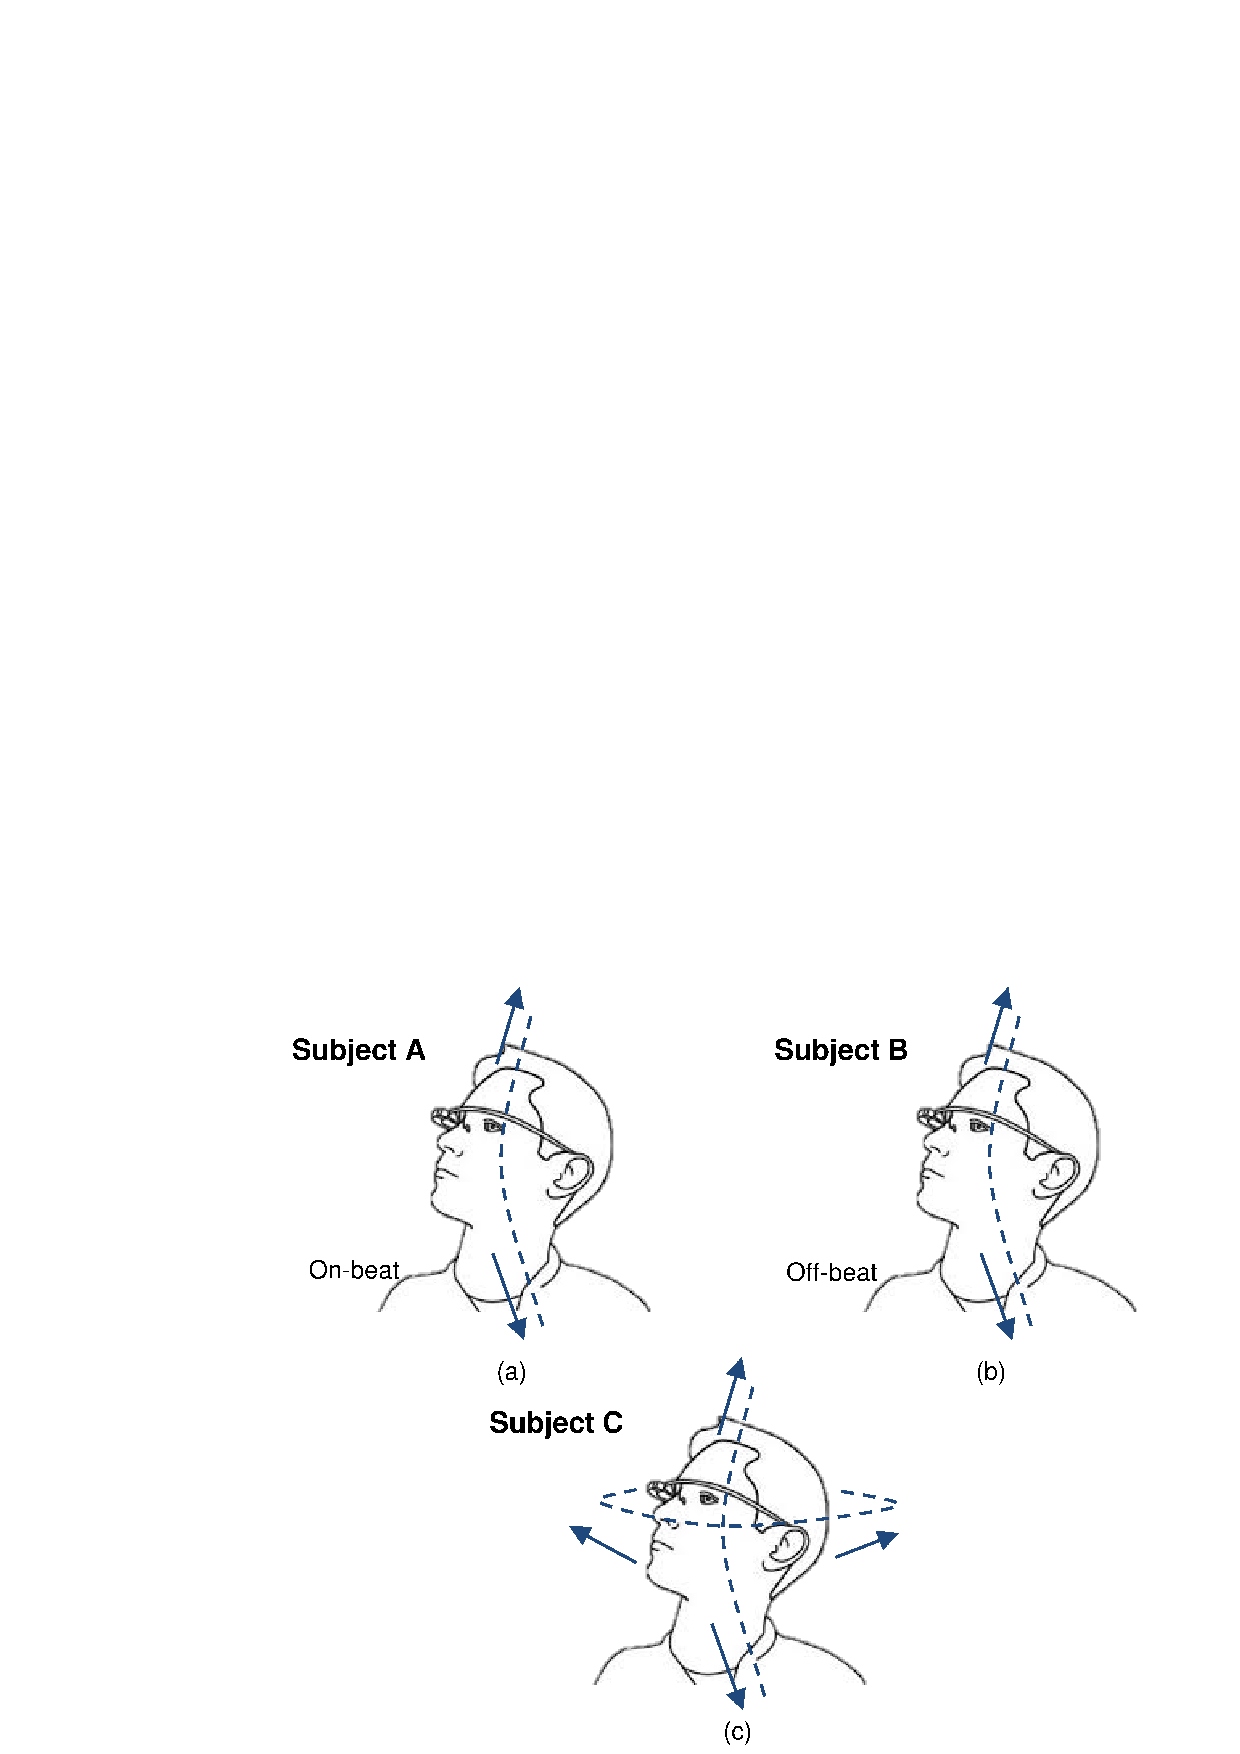
\includegraphics[width = \columnwidth]{figure/imitation_subject_movement.png}
\caption{\label{fig:imitation_movement} Pictorial description of how the mimicked subjects move.}
\end{figure}


\subsection{Authentication Robustness of \systemname} After evaluating authentication accuracy for \systemname, we next study its robustness. In this study, we focus on imitation attacks. For this purpose, we asked a number of subjects (attackers) to imitate simple nodding patterns from three subjects (targets) after watching the target's video for as long as they desire, and calculated their chances of successful imitation - i.e., the attacker is mistakenly accepted by \systemname. We note that nodding is the simplest head-movement pattern and easiest to imitate; hence, the results presented here represent the \emph{lower bound} robustness that \systemname~offers. In reality, users are more likely to employ more sophisticated head-movement patterns, which will be much harder to imitate.

\subsubsection{Participants}
We had a total of 37 volunteer participants, including 31 males and 6 females. The average age of the participants was 25.6 years with a standard deviation
of 6.6 years. The youngest participant was 22 years old while the eldest was 49 years old.

\subsubsection{Procedure}
Our second experiment aimed at emulating a practical imitation attack scenario. In this experiment, three targets recorded video when they were nodding with a music cue. Note that the music is usually played via a bone conduction speaker or an earplug, and that it is difficult to use a camcorder to capture the music sound in a noisy environment. To address this concern, during recording, we set the speaker volume to maximum and conducted the recording in a quiet laboratory environment.

We divided the attackers into three groups, and asked each group to imitated one target. In each session (consisting of 30 trials), the attacker could watch the video for as long as they wish. Our system provided a feedback after each trial so that the attackers could adjust their nodding pattern if they wanted. After the attacker had 30 trials,
we ended the session no matter whether the attacker had succeeded or not. In each session, we noted the total number of successes the attacker had as well as the number of trails before the first successful imitation. %This experiment was conducted in quite space on campus. We will now discuss our evaluation results for both experiments in detail.

\subsubsection{Results}
Each of the three targets performed simple nodding in this experiment; though simple, their nodding patterns have varying complexity. As shown in Figure~\ref{fig:imitation_movement}, Target $A$ moved his head vertically, each nodding on a music beat, with no noticeable horizontal movement; target $B$ also only moved his head in the vertical direction, but there was always a delay between his nodding and the corresponding music beat; target $C$ combined slight shaking along with nodding, and closely followed music beats. Among these three targets, $A$ is the easiest, while the other two are slightly more complex.

Table~\ref{tab:imitation} summarizes the results. Here, we use FAR to denote the successful imitation rate because a successful imitation is counted as a false acceptance in our system. The overall FAR of the experiment is 6.94\%, while the individual FARs for the three targets are 15.83\%, 2.77\% and 2.72\% accordingly.  Since target $A$ had the easiest nodding pattern, 7 out of 12 subjects could succeed at least once during their 30 trials, while for targets $B$ and $C$, the numbers are  3 out of 13 and 3 of 12, respectively. These results are very promising: when a user employs slightly more complex head-movement patterns, it becomes much harder for others to imitate (EER dropping from more than 15\% to around 2.7\%).



\begin{table}[b]
\centering
\begin{tabular}{|l|c|c|c|c|}\hline
                               & No. &  No. &  Average No. of  &  \\
Target & of & of & Trials Before & FAR (\%) \\
& Attackers & Successful Attackers & First Successful Login & \\\hline

A                   & 12                                 & 7                                                                     & 10.33                                                                                               & 15.83                        \\ \hline

B                   & 13                                 & 3                                                                     & 14.33                                                                                               & 2.77                         \\ \hline

C                   & 12                                 & 3                                                                     & 17.67                                                                                               & 2.72                          \\ \hline\hline

Overall & 38                                 & 13                                                                    & 13.17                                                                                                    & 6.94                         \\ \hline
\end{tabular}

\caption{\label{tab:imitation} The attack results show that as head-movement patterns become more complex, it becomes much harder to imitate. }

\end{table}



\subsection{Headbanger Google Glass App Implementation}\label{subsec:app}

\begin{figure}[t]
\centering
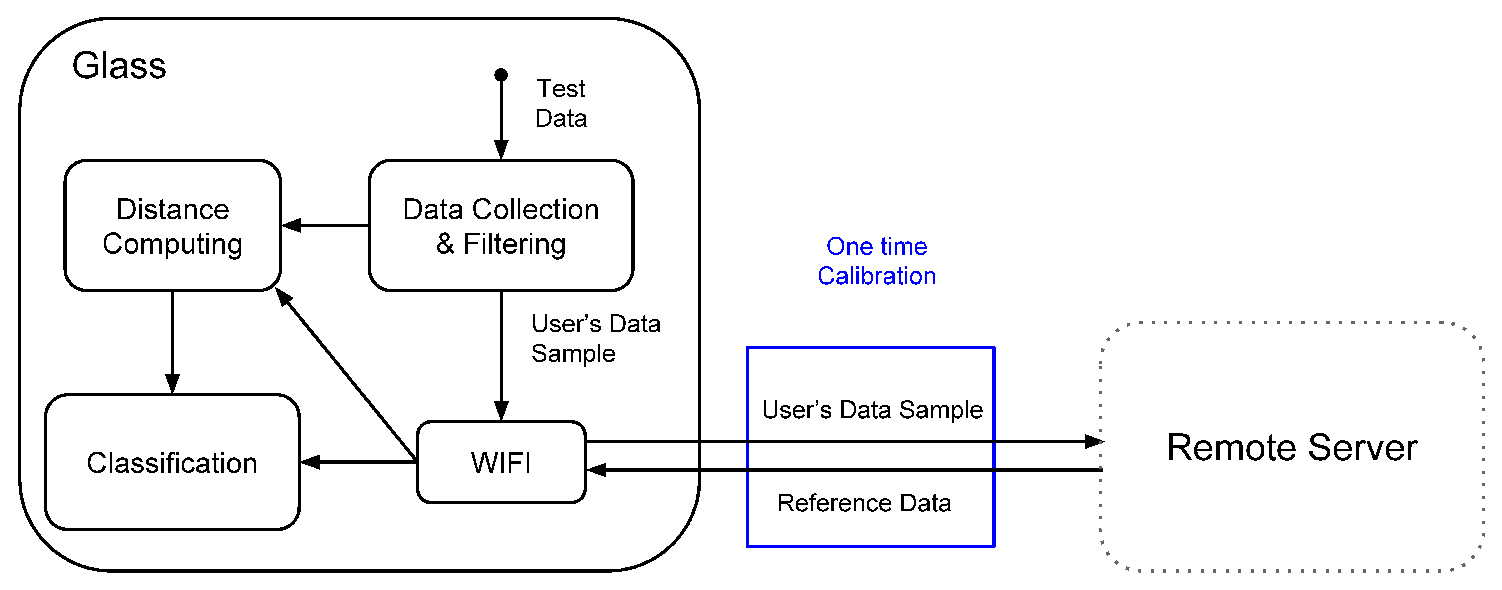
\includegraphics [width=\columnwidth]{figure/software_arch.eps}
\caption{Software modules of \systemname~implementation}
\label{fig:glass-softwarearch}
\end{figure}

In the second phase of evaluation, we implemented \systemname~on Google glass
as an authentication app.
Figure~\ref{fig:glass-softwarearch} shows the main software modules in the
app. Upon initiation by the user, the app plays a music cue for a user-specified
duration. The user conducts head-movements in synchrony with the music cue
while the app records the accelerometer data in parallel. At the end of the
music cue duration the app enters the data processing phase where the
sensor readings are input to the \systemname's software modules for
processing. %The processing stage includes the filtering of the accelerometer
%sensor values, classification and feature extraction using DTW, and threshold
%based matching of the generated features with those from training set.
%%\systemname extracts the head-movement features through
%%the thresholding process discussed in section~\ref{sec:design}, and compare
%%with the feature templates generated from the training phase.
Upon completion of data processing, the app responds with a YES or NO textual
output on the Google Glass screen. The training phase is conducted offline on a PC, and %prior to live-testing off the application.
%The training phase
%which involves collecting 30 samples of the
%head-movement accelerometer readings, generating the features, and saving them
%into a local server (running on PC) as an XML file, with appropriate indexing.
%Upon app initiation on Glass, the trained features are pre-fetched from
%the server through a wireless connection.
we ensure that the training set
is readily available during the authentication process. %thus eliminating the
%additional processing time required for the training phase.
%Conducting online training, particularly that involves DTW computations, is
%very compute intensive on a resource constrained devices such as Glass.
%One possible solution would be for the Glass to offload the
%training phase computation to a local server machine.
%We reserve such considerations for future implementations.

%Among all the software modules, the ``training set construction model'' is
%the most computing-intensive, and as a result, we executed the model on the
%bluetooth-paired smartphone. The rest of the modules are implemented and
%executed on the glass.
%In our on-glass app, the classification module runs the
%thresholding-based classification.
\subsubsection{Data Processing Latency}

\begin{table}[b]
\centering
\begin{tabular}{|ccclc|}
\hline
\multicolumn{1}{|c|}{\multirow{2}{*}{\begin{tabular}[c]{@{}c@{}}music  cue \\
duration (s)\end{tabular}}} &
\multicolumn{1}{c|}{\multirow{2}{*}{\begin{tabular}[c]{@{}c@{}} data processing latency (s)\end{tabular}}} & \multicolumn{3}{c|}{time breakdown (\%)}
\\ \cline{3-5}
\multicolumn{1}{|c|}{}
                             &
\multicolumn{1}{c|}{}
                              &
 Filtering & \multicolumn{1}{c}{DTW} & Thresholding   \\
 \hline\hline
10
                             &
1.93
                              &
 0.49      & 99.50                   & 0.01  \\
6
                             &
1.15
                              &
 0.63      & 99.36                   & 0.01  \\
5
                             &
0.88
                              &
 0.82      & 99.19                   & 0.01 \\ \hline
\end{tabular}
\caption{\label{tab:glass} Measured response time of \systemname~app implementation on Google
Glass with different music cue durations and for $K = 1$. The response time
reported here is an average over 20 trials.}

\end{table}

In Table~\ref{tab:glass} we report the measured average processing latency
of the \systemname~app for music cue durations
of 5, 6 and 10 seconds. %We conducted the benchmark execution-time profiling of
%\systemname~on Glass in a controlled indoor laboratory setting with no
%mobility. We define response time as the time elapsed between music cue
%completion to
%the display of authentication response (YES/NO text) on the Glass screen.
The processing latency is within 2 seconds for a 10-second data input, and is less than 1 second (0.88s) for a 5-second input.
%We feel that a response time of 2-5 sec for a local authentication solution in
%Google Glass is comparable to that of prior-art that comes close to our
%solution~\cite{von2013patterns,egelman2014you}.
%It is important to note that authentication solutions that execute
%locally on head-worn wearable devices, especially on a heavily resource
%constrained device like Glass, are still not mature. However, the hope is that
%such solutions will possibly catch up to speed in the near future and that our
%approach is advancing one step in that direction.
We also report the total latency breakdown for different software modules, and find that DTW computation is the main bottleneck. In our implementation, we used Fast DTW~\cite{salvador2007toward} which decreases the computation complexity from $O(n^2)$ to $O(n)$  without compromising the authentication accuracy.
%We can observe from Table~\ref{tab:glass} that the DTW computation
%dramatically compute intensive than the other processes.

As we discussed earlier, the processing latency can be further reduced, and it could be partially hidden if we pipeline the data processing and data input. As a result, we believe that our design of \systemname~is indeed \emph{light-weight} and it is realistic to run the \systemname~app on devices that have comparable computing capabilities as the Google Glass.
%It is important to note that our current implementation uses a faster
%version of the DTW algorithm called Fast DTW~\cite{salvador2007toward},
%providing about 2x speed-up in DTW computation.
%We believe that the response time can be reduced
%further through strategic methods such as, further optimizations in the Fast
%DTW algorithm or pipelining the app execution along with data collection.
%A specific strategy for reducing response time for rejected attempts can be
%that, after a short duration, before the entire music cue is played, if it is
%found that a user's movement does not match the signature of the claimed user
%with a sufficient pre-determined confidence level, then the on-site
%classification may be terminated instead of waiting for the entire duration to
%yield the rejection.
%Another example, may include cyber-foraging strategies to offload heavy
%computation tasks, such as online training and classification, to the user's
%Bluetooth paired smartphone or a nearby cloudlet~\cite{ha2014towards}.

 
\section{Discussion and Future Work}\label{sec:disc}

In this study, we showed that head-movements have the potential to be used as
a reliable biometric characteristic for user authentication.
We will now discuss some of the limitations that we identified from this work
and prospects for future work as below.

\subsection{Reliability}
Our work in this paper shows that head-movements are distinctive and
repeatable in controlled settings. However, in reality, the behavior of
head-movement signatures over chaotic settings will be a key factor to decide
on the effectiveness of this approach. Our work only evaluates the case when a
user is in a stationary setting when attempting to login, such as when sitting
on the chair or standing still. The performance of this approach in realistic
mobile settings such as walking or in a vehicle is yet unknown. It is also
unclear if the head-movement patterns are repeatable in such a mobile environment, or
if the ambiguities of vehicle motion versus head-motion can be separated. 
%%For example, we don't know whether a person's
%%head-movement signature will be the same no matter whether she is sitting,
%%standing still, walking, running, or driving.
%%The most important concern is the reliability of human head-movements. Even
%%though we have shown that head-movements are rather distinctive and
%%repeatable
%%in a controlled setting, it is yet unclear how it will perform in realistic,
%%but chaotic settings. For example, we don't know whether a person's
%%head-movement signature will be the same no matter whether she is sitting,
%%standing still, walking, running, or driving.
Similarly, a person's head-movement signature may also depend on the mood/energy level of
the person; for example, a fresh and energetic user may provide significant
head-movements as compared to a sick or tired user whose signatures may not
even be detectable. Inconsistencies in the accelerometer sensor such as drift and temporal bias can
significantly affect the nature of inferred head-movement signature.
Head-movements, on the other hand, may also evolve over time for a person
which call for periodic calibration of the system and/or the training data.
%To address these two temporal changes, we may need to periodically
%recalibrate
%the sensors and dynamically adjust our training data to reflect new movement
%trends.

While reliability metric was out of the main scope of this paper, we are keen
to address the same in future work.

\subsection{Multi-Modality}
Smart-glass devices typically contain an array of motion sensors such as accelerometer, gyroscope, IMU. It is only a matter of time that motion sensor chips will be integrated into wearable devices.
This opens up opportunities for multi-modal motion sensing. For example,
accelerometer data can be combined with gyroscope measurements to provide
multi-dimensional head-movement features that can improve the quality of the
inferred signatures. Head movements can also be combined with other body movements to generate
valuable, reliable signatures for authentication. 
%Additionally, head-movement is just one type of body movements, and we can
%investigate other types of body movements as well.
For example, through a simple test experiment using the Google Glass
infra-red light sensor\footnote{we had to root the Google Glass to access the
IR sensor unit.} we observed that the blinking and winking patterns of users in
response to the music stimulus were reasonably differentiable among users.
Such patterns may also independently serve as another biometric that can be
used for authentication purpose, or can be combined with head-movements for better results.
Recent studies have shown that heart beat or pulse can also serve as reliable
biometric for authentication purposes~\cite{hernandezbioglass,nymi}
We reserve such potential enhancements to our system for future implementation.
%A recent study has shown that Google glass can detect human heart
%beat~\cite{hernandezbioglass}; heartbeats can thus be
%used as another biometric.
%If extra hardware can be introduced, then more movement patterns,
%such as eye movement, can be leveraged as well.

\subsection{Seamless Protocol}
An authentication system must have an effective protocol for authenticating
users seamlessly to their device. Our system runs a simple authentication
protocol where the user is given a finite set of (calibrated) music
tracks to pick, and based on which the user makes head-movements in response.
Our design assumes that the user voluntarily accepts the enforcement of the
requirement of head-movements in response to the music. A seamless design
would ensure that the system captures even the slightest of the subconscious
head-movements in the event that the user does not make any enforced
head-movements. In such cases the head-movement signatures will have to be
much more elaborate with multiple attributes that correspond to the different
realistic use-cases of the system.
%Our protocol can consist of several steps. In the first step, the user will
%be
%asked to choose a user name from all the legitimate users of the device.
%Then,
%the user will be asked to select the favorite music track of the claimed
%user.
%If the selection is correct, the device will play the music and ask the user
%to move along (including head movement, eye blinking/winking, etc). ***YZ:
%what else??? ***

\subsection{Processing/Battery Power Constraints}
Battery power consumption and computing power are very important parameters
for consideration when optimizing a design to accommodate to wearable devices.
Wearables usually have serious resource limitations, especially in terms of
processing power and battery power.
This paper, addresses these concerns through optimization strategies in the
head-movement signature classification stage of the proposed authentication
algorithm. For wearables it is important that such optimization strategies are
taken to next levels until a roadblock is reached.
%In this paper, we have considered a set of
%optimization techniques to reduce the processing demand as well as power
%consumption, e.g., testing against top $K$ samples instead of  the entire
%training set, using thresholding-based classifier instead of SVM classifier.
For example, one such strategy extension in this work can be that, after a
short duration, before the entire music is played, if it is found that a
user's movement does not match the signature of the claimed user
with sufficient confidence level, then the on-site classification may be
terminated  instead of waiting for the entire duration to yield the rejection.
Another example, may include cyber-foraging strategies to offload heavy
computation tasks, such as classification, to the user's Bluetooth paired
smartphone.

\subsection{Large-scale evaluation}
To be adopted as a primary authentication mechanism on smart-glass devices,
the technique will have to be evaluated over a large number of usage and
and over a large user base. Conducting such rigorous large-scale experiments
are typically infeasible in academic laboratory settings. We reserve such
large scale experiments for future work, and hope to accomplish through
industry collaborations.

\section{Related Work}\label{sec:related}
Headbanger is a 3D behavioral biometric based
activity recognition system, which focuses on head movement in this paper. 
To our best knowledge, it is the first wearable authentication system that only relies on
accelerometer signatures from human \emph{head} motion. Below, we briefly review the related literature on mobile device authentication.

%in wearable/mobile device based schemes, infrastructure based
%schemes, and biometric-rich based schemes.

%\subsection{Wearable/mobile device based schemes}
Harwin et al.~\cite{harwin1990analysis} was considered the first that
proposed to use head gestures by combining pointing and movements
for human computer interaction. The closest work to ours is
the one in~\cite{westeyn2004recognizing}, in which eye
blinking pattern was used as a unique feature for
authentication. They achieved 82.02\% accuracy with 9 participants. Compared to eye blinking pattern, head-movements provide much more entropy, therefore a more suitable biometric characteristic. 
Ishimaru et al.~\cite{ishimaru2014blink} proposed to combine the eye blinking frequency from the infrared proximity sensor and head motion patterns from accelerometer sensor on Google Glass
to recognize activities (e.g., reading, talking, watching TV,
math problem solving), and achieved 82\% recognition
accuracy. While their approach looked at common patterns when people employ the same activities, ours took a deeper look at the head-movements and found that everyone's head-movements are unique. There are also a number of head
motion based activity recognition studies using computer vision, such
as the one in~\cite{kjeldsen2001head}. BioGlass~\cite{hernandezbioglass}
combines Google Glass's accelerometers, gyroscope, and camera to
extract physiological signals of the wearer such as pulse
and respiratory rates.

Accelerometers have also been used to measure movements in other part of the
body for gait-based authentication purpose, such as
waist~\cite{ailisto2005identifying}, pocket~\cite{gafurov2007gait},
arm~\cite{okumura2006study,gafurov2008arm},
leg~\cite{gafurov2006biometric} and ankle~\cite{gafurov2011user}.
They are similar in that they collect the raw accelerometers data
and apply signal processing and/or machine learning techniques  to perform
authentication.

Hand gesture and touchscreen dynamics are often coupled for
authenticating that device. A number of contextual features
including biometrics (e.g. finger length, hand size,
swipe/zoom speed, acceleration, click gap, contact size, pressure)
and behavioral feature (e.g. touch location, swipe/zoom length,
swipe/zoom curvature, time, duration) have been exploited as
effective features for authentication purpose such as demonstrated
in~\cite{sae2012biometric,frank2013touchalytics,cai2013mobile,feng2014tips}.
While most of the techniques require users to explicitly conduct a
gesture following a specific pattern, TIPS~\cite{feng2014tips}
proposed a multi-stage filtering with dynamic template adaptation
strategy to perform the user authentication in a uncontrolled
environments -- as user naturally use the phone. There are a number of
authentication schemes using techniques such as
speech~\cite{reynolds2000speaker}, computer vision and image
~\cite{bowyer2006survey}, graphical
password~\cite{biddle2012graphical,sherman2014user}, biometric
fingerprints~\cite{jain1997identity}. 


Finally, we take the viewpoint that our approach can be used as a complementary scheme to most
of the existing techniques.

%It was extended by Kjeldsen~\cite{kjeldsen2001head} to more
%categories such as continuous control, spatial selection and
%symbolic selection

%Gafurov et al.~\cite{gafurov2006biometric} developed a wearable
%biometric gait authentication system. The sensor is attached to the
%lower leg to extract the gait patterns -- accelerations in three
%directions: vertical, forward-backward and sideways motion of the
%lower leg. A combination of these accelerations is used for
%authentication. ~\cite{gafurov2011user} ankle
%\subsection{Infrastructure based schemes}

%\subsection{Biometric-rich based schemes}
%Fingerprints

% are we the first one? the cloest work? how far we are going to reach out? categories in general: image? voice? touch?
% on glass; body movement;

%mobisys 2014 papers

%gesture based authentication

%Music based movements -- GaTech

%Japanese paper on google glass and eye-wink

%hardware fingerprinting -- check CCS 2014

%acc-based authentication
%http://ieeexplore.ieee.org/xpl/articleDetails.jsp?arnumber=5634532&sortType%3Dasc_p_Sequence%26filter%3DAND%28p_IS_Number%3A5634461%29

%wearable security
%http://gaia.cs.uiuc.edu/papers/wss.pdf

%commercial solutions: Nymi -- eyewink blink pattern

%BioNym -- heartbeat

\section{Concluding Remarks}
\label{sec:conc}

We developed a system that uses head-movement patterns of users for direct
authentication to a wearable device. We developed a light-weight approach that infers
head-movements of users in response to music and generates signatures
that are unique to every user.
Experimental observations revealed that the head-movement signatures generated
using the dynamic time-warping tool, in response to the same music track, were
consistent in typical stationary environments such as user sitting or
standing at one location while attempting to authenticate. We leveraged the
consistency in the head-movement signatures to develop two classification
algorithms, based on machine learning and adaptive thresholding, to
efficiently and accurately label user signatures.
Through a multiple user based experiment evaluation using the data collected
by our sensor data collection app in Google Glass, we observed that the
average true-acceptance rate of our approach is above 95.1$\%$ and the false
detection rates is below 4.43$\%$. We have also optimized our algorithms to minimize the processing latencies and power consumption, making them suitable for wearable devices.
The multi-user training data sets were validated and verified during the
course of our evaluations and will be released for public use in near future.

\iffalse
In this paper, we present the design, implementation and evaluation
of Headbanger, a head gesture based authentication system.
Headbanger generates a signature from user's head-movements in
response to short duration of audio track with fast beats, and uses
this signature as the behavioral biometric for authentication.
Through extensive experiments on the prototype on Google Glass
involving ?? users, we demonstrated that Headbander can achieve **\%
accuracy and thus with proper audio stimuli, head-movement alone
will be reasonably sufficient to serve a effective behavioral
biometric for authentication. We believe this work will be the basis
for using audio catalyst to enrich more useful human contextual
applications.
\fi

\balance
%\scriptsize
%\footnotesize
%\small
%\bibliographystyle{acm-sigchi}
\bibliographystyle{abbrv}
\bibliography{sugang}
\end{document}
